\chapter{Appendix B: Top Results}
\label{appendixB}

Here we show the signal and background distributions for the input variables used for training the BDT for our top analysis. In all cases the plots are normalised to unity and show the raw distributions before preselection cuts are applied. Efficiencies for the lower $\sqrt{S'}$ bins following each stage of selection are also shown. 


\begin{figure}[] 
  \begin{subfigure}[b]{0.5\linewidth}
    \centering
    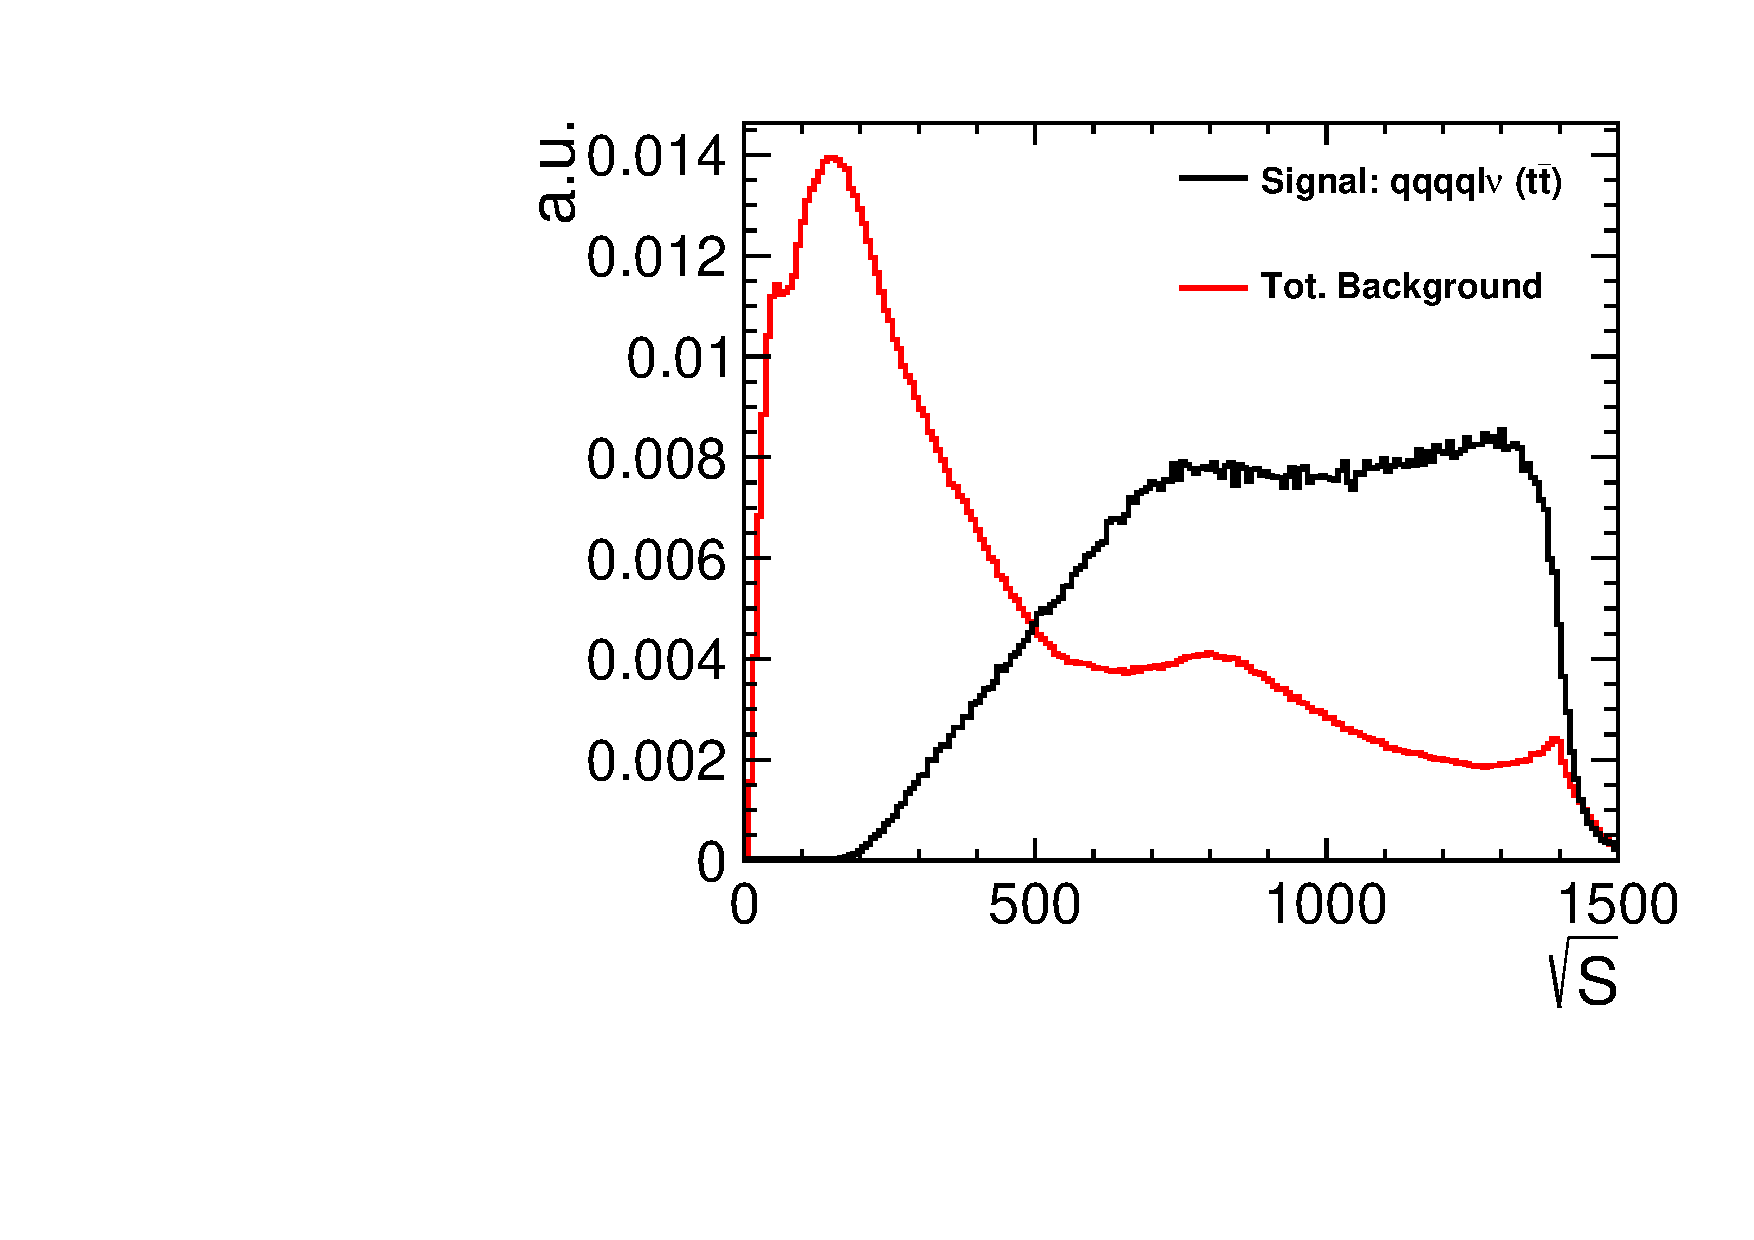
\includegraphics[width=0.75\linewidth]{TopAnalysis/figures/BDTVariables/EnergyConstraintAlt} 
    \caption{Centre of mass} 
    \vspace{4ex}
  \end{subfigure}%% 
  \begin{subfigure}[b]{0.5\linewidth}
    \centering
    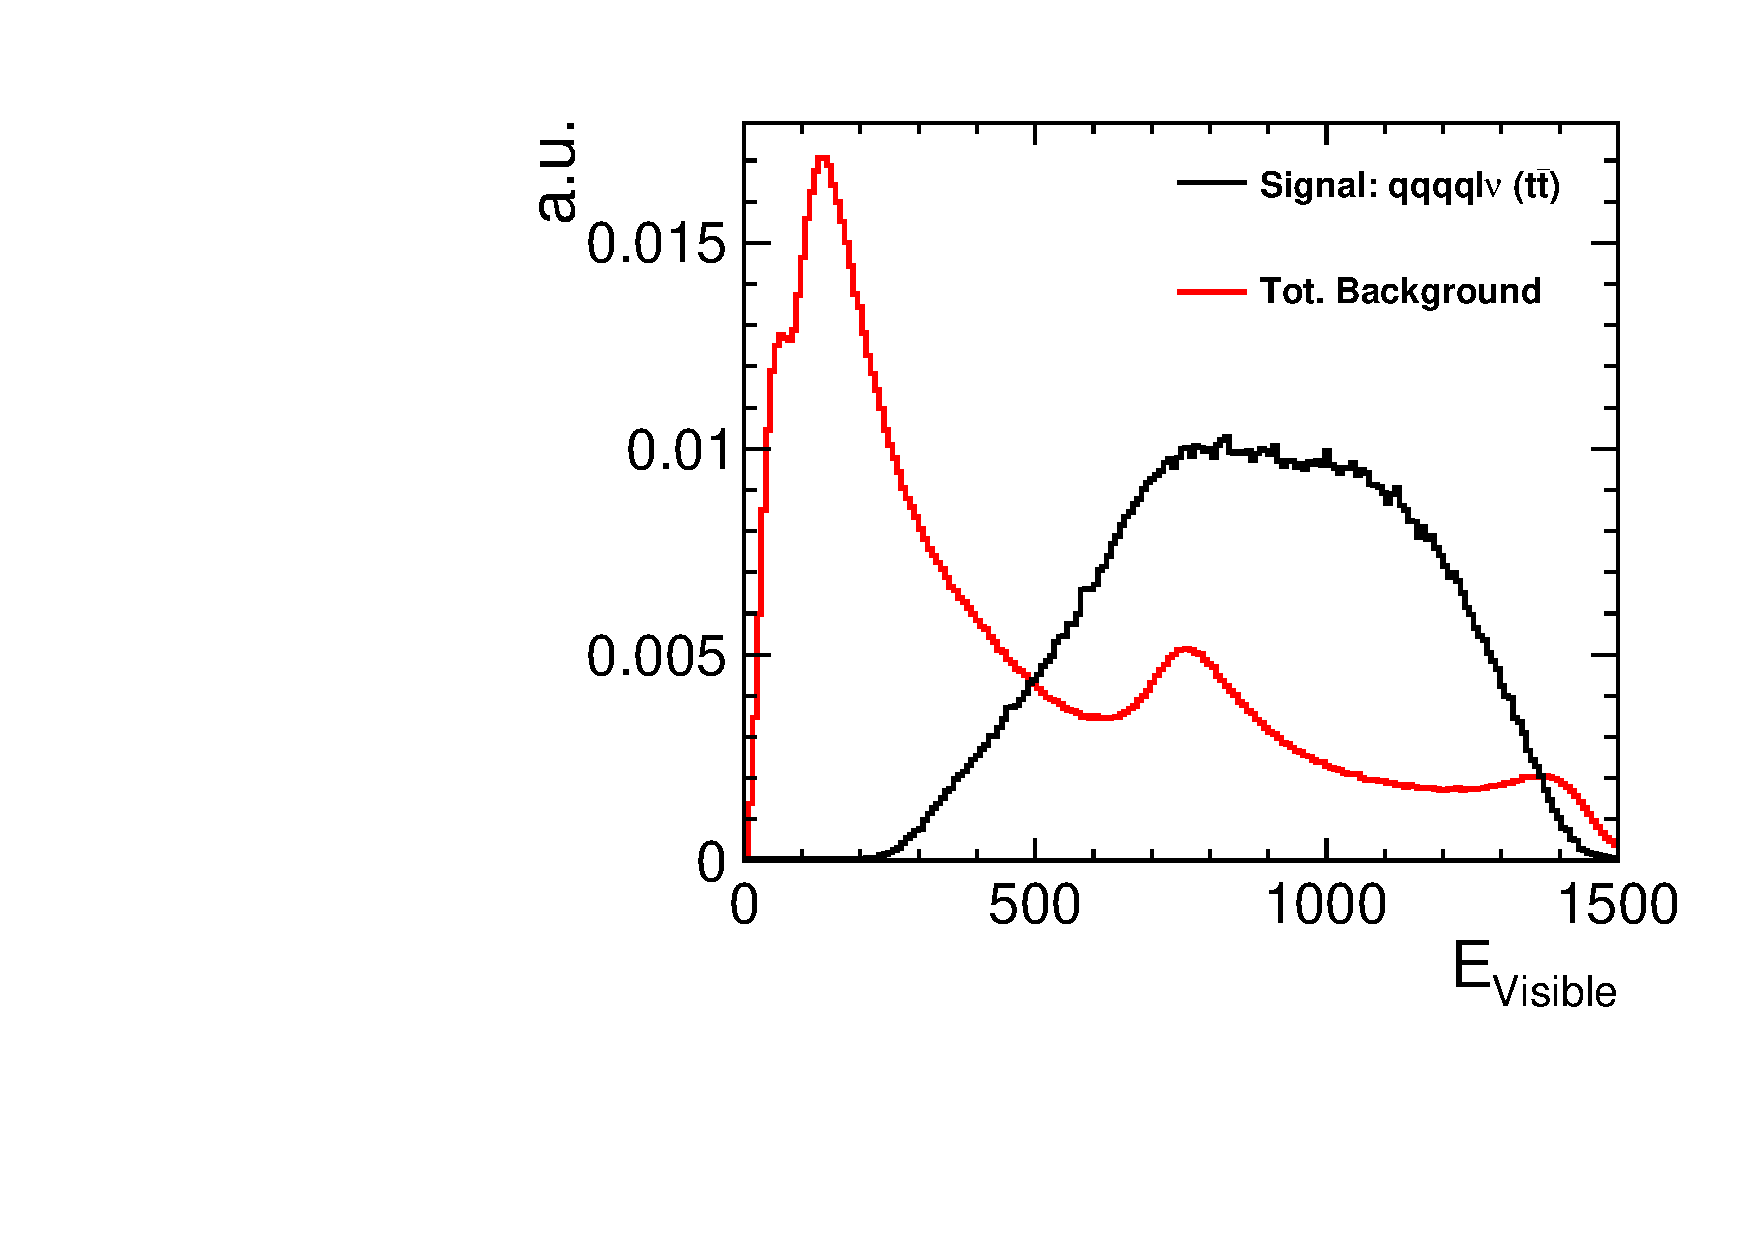
\includegraphics[width=0.75\linewidth]{TopAnalysis/figures/BDTVariables/VisibleEnergy} 
    \caption{Visible Energy} 
    \vspace{4ex}
  \end{subfigure} 
\end{figure}

\begin{figure}[]\ContinuedFloat 
  \begin{subfigure}[b]{0.5\linewidth}
    \centering
    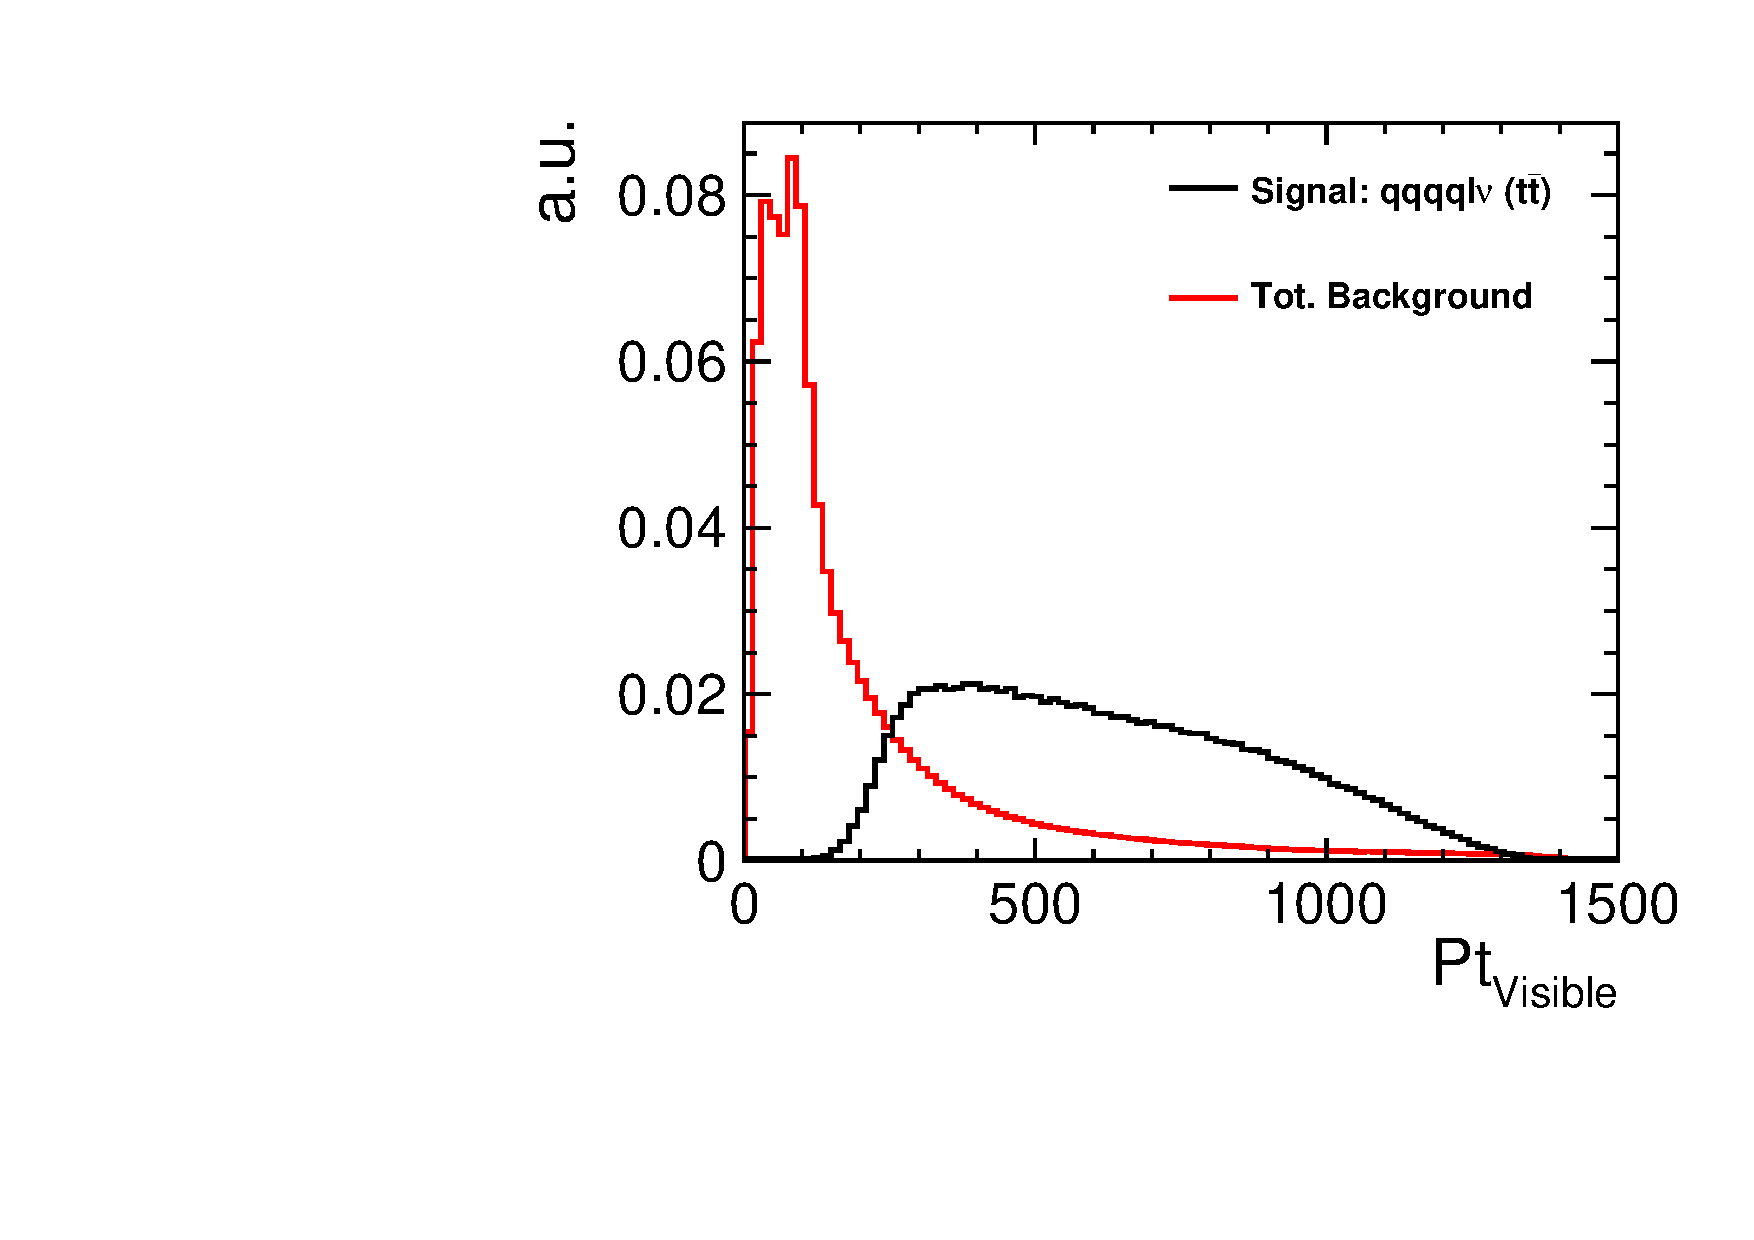
\includegraphics[width=0.75\linewidth]{TopAnalysis/figures/BDTVariables/VisiblePt} 
    \caption{Visible Transverse Momentum} 
    \vspace{4ex}
  \end{subfigure}%% 
  \begin{subfigure}[b]{0.5\linewidth}
    \centering
    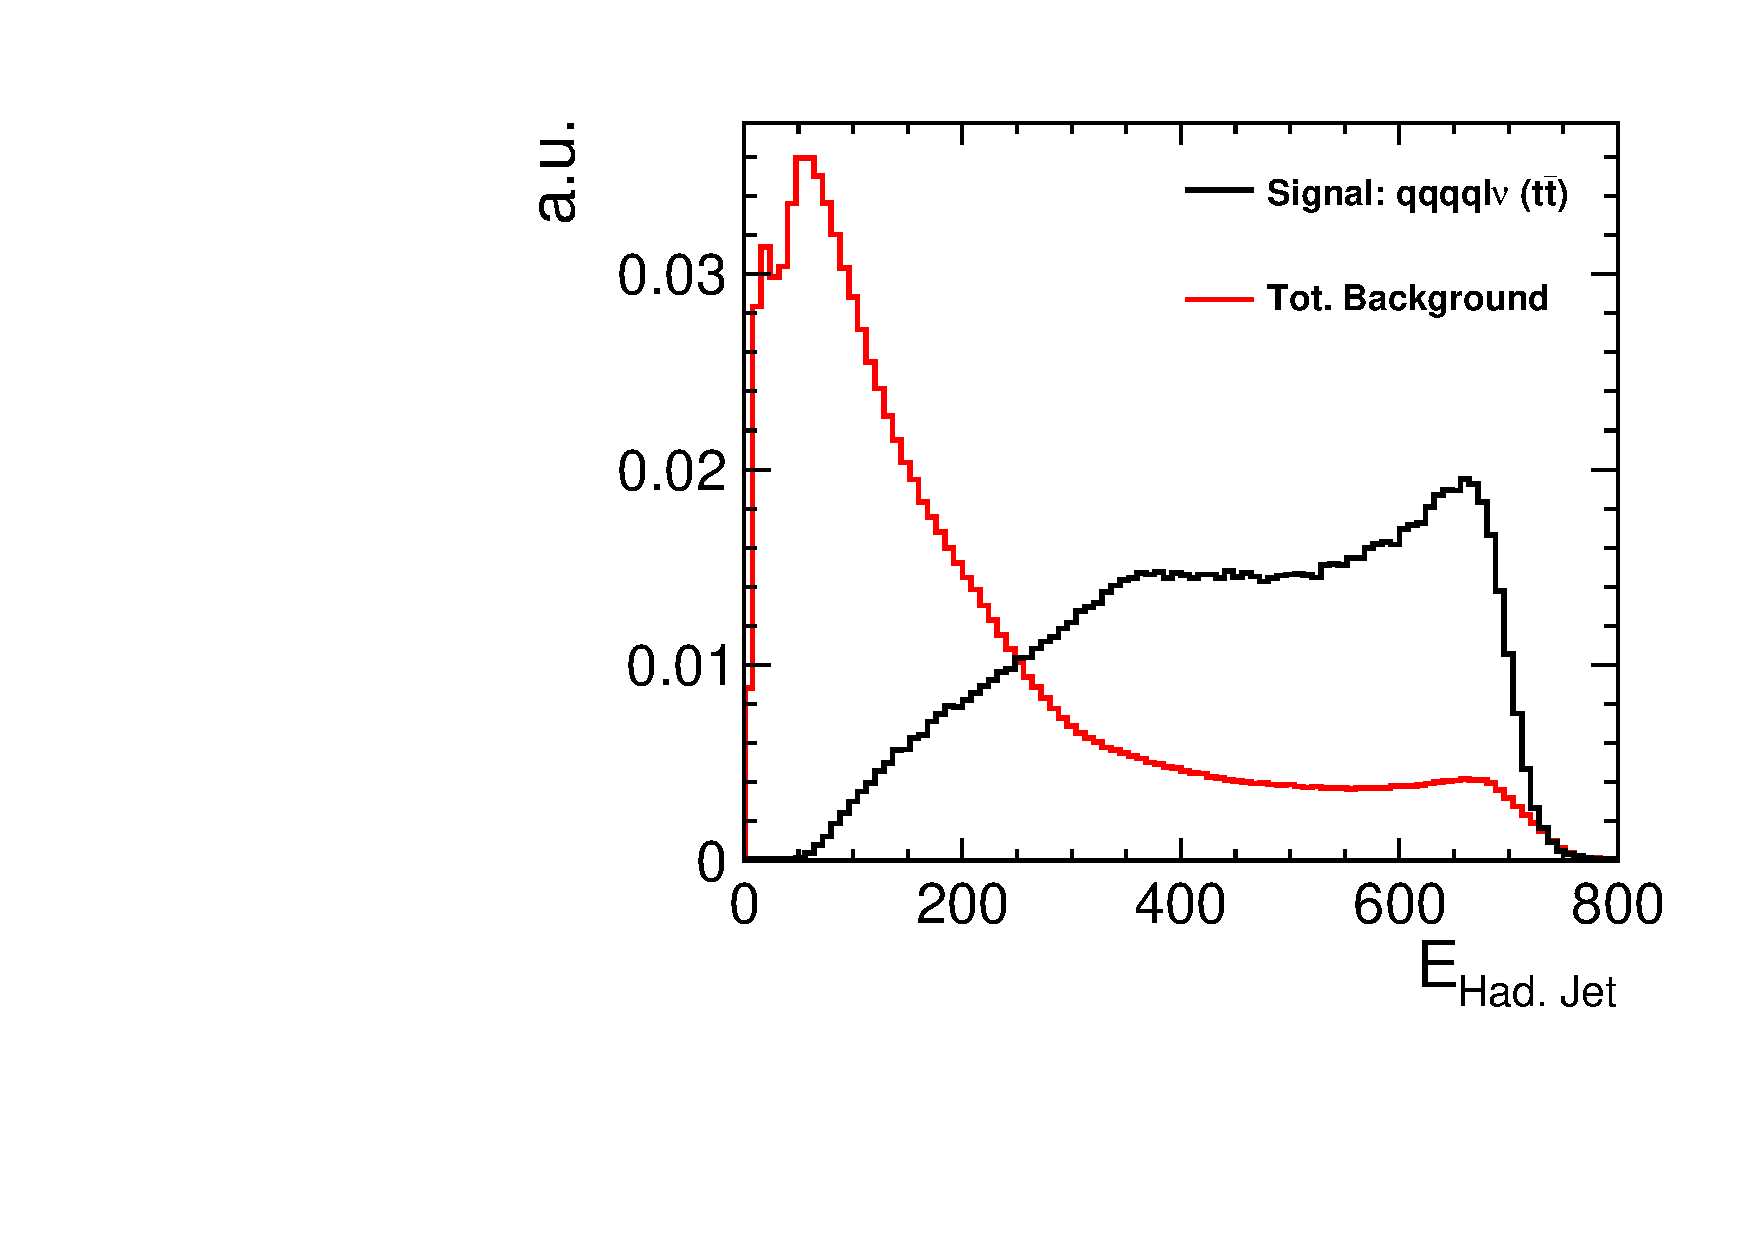
\includegraphics[width=0.75\linewidth]{TopAnalysis/figures/BDTVariables/HadronicEnergy.pdf} 
    \caption{Energy of hadronic fat jet} 
    \vspace{4ex}
  \end{subfigure} 
  \begin{subfigure}[b]{0.5\linewidth}
    \centering
    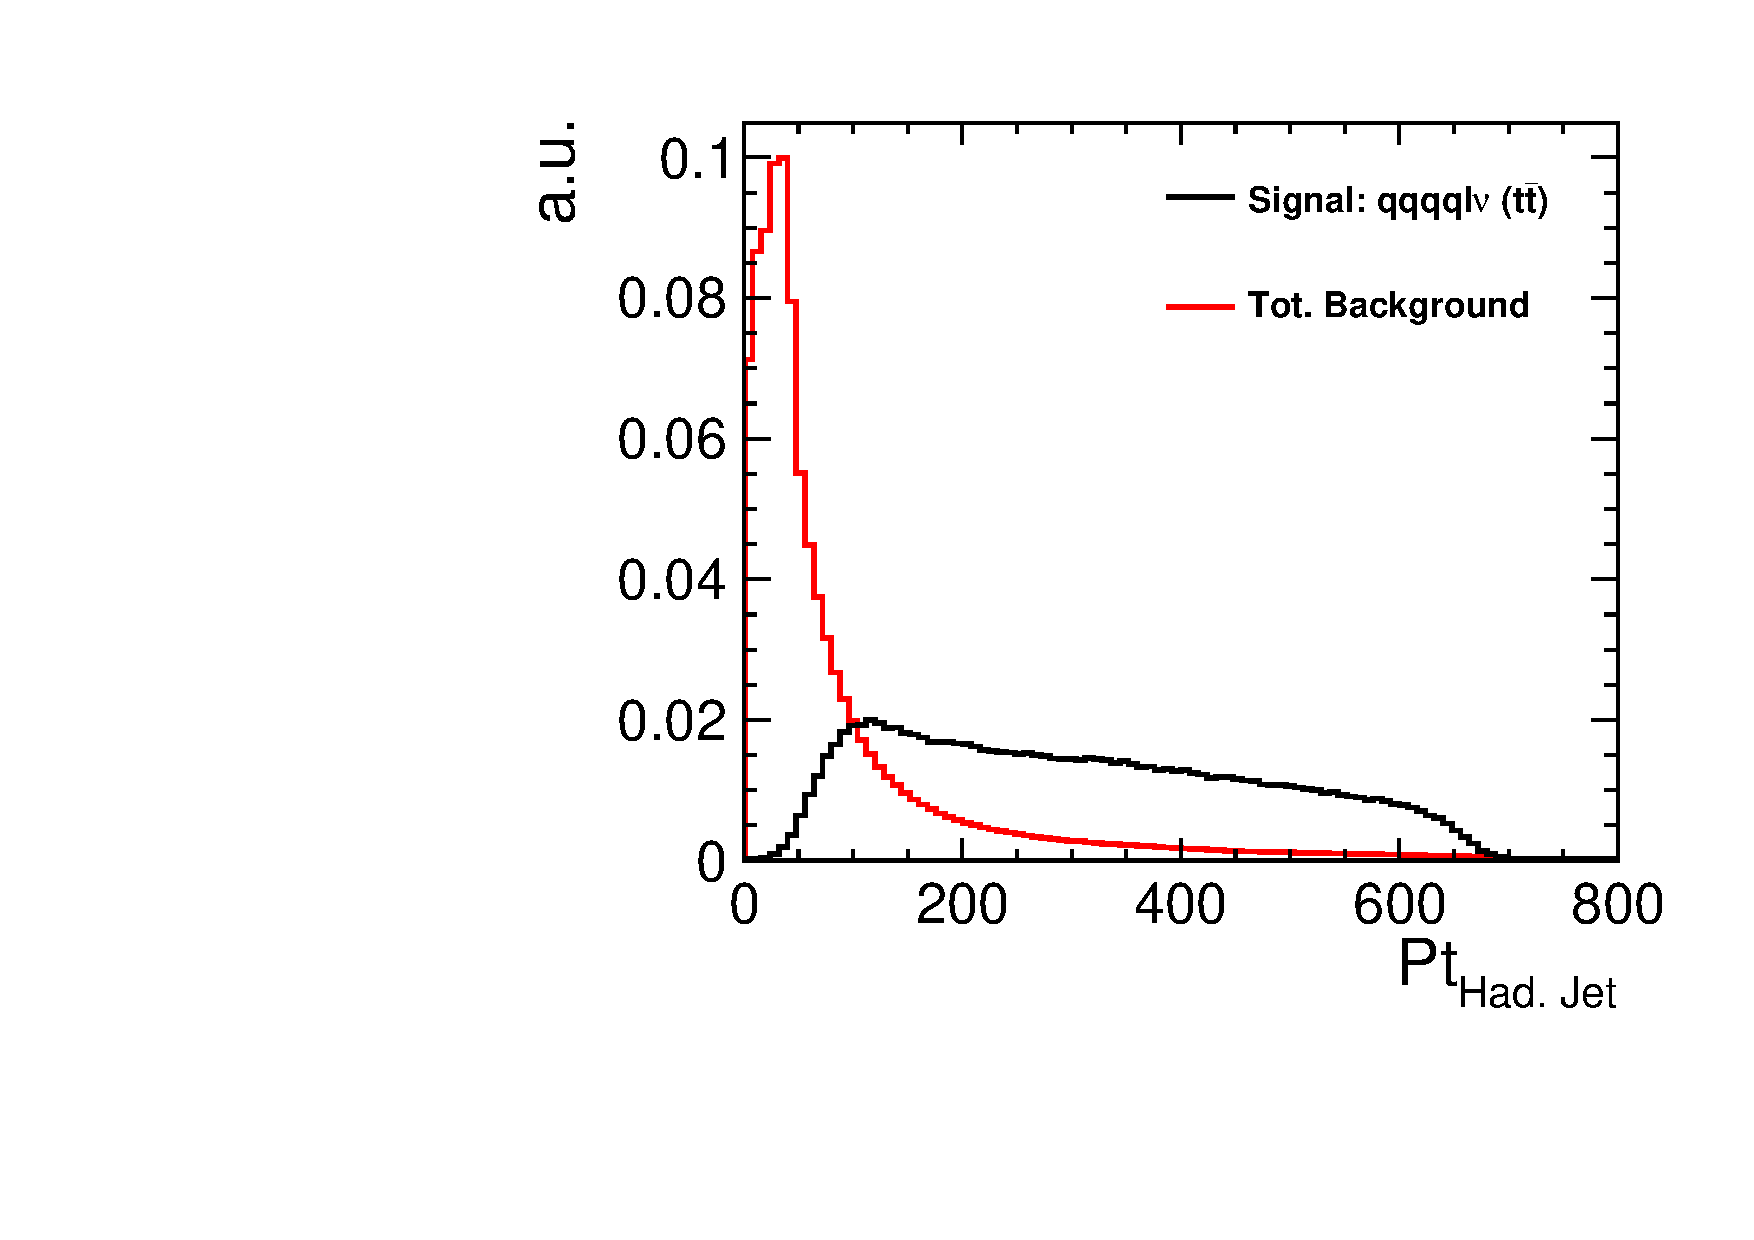
\includegraphics[width=0.75\linewidth]{TopAnalysis/figures/BDTVariables/HadronicPt.pdf} 
    \caption{Transverse momentum of hadronic fat jet} 
    \vspace{4ex}
  \end{subfigure}%%
  \begin{subfigure}[b]{0.5\linewidth}
    \centering
    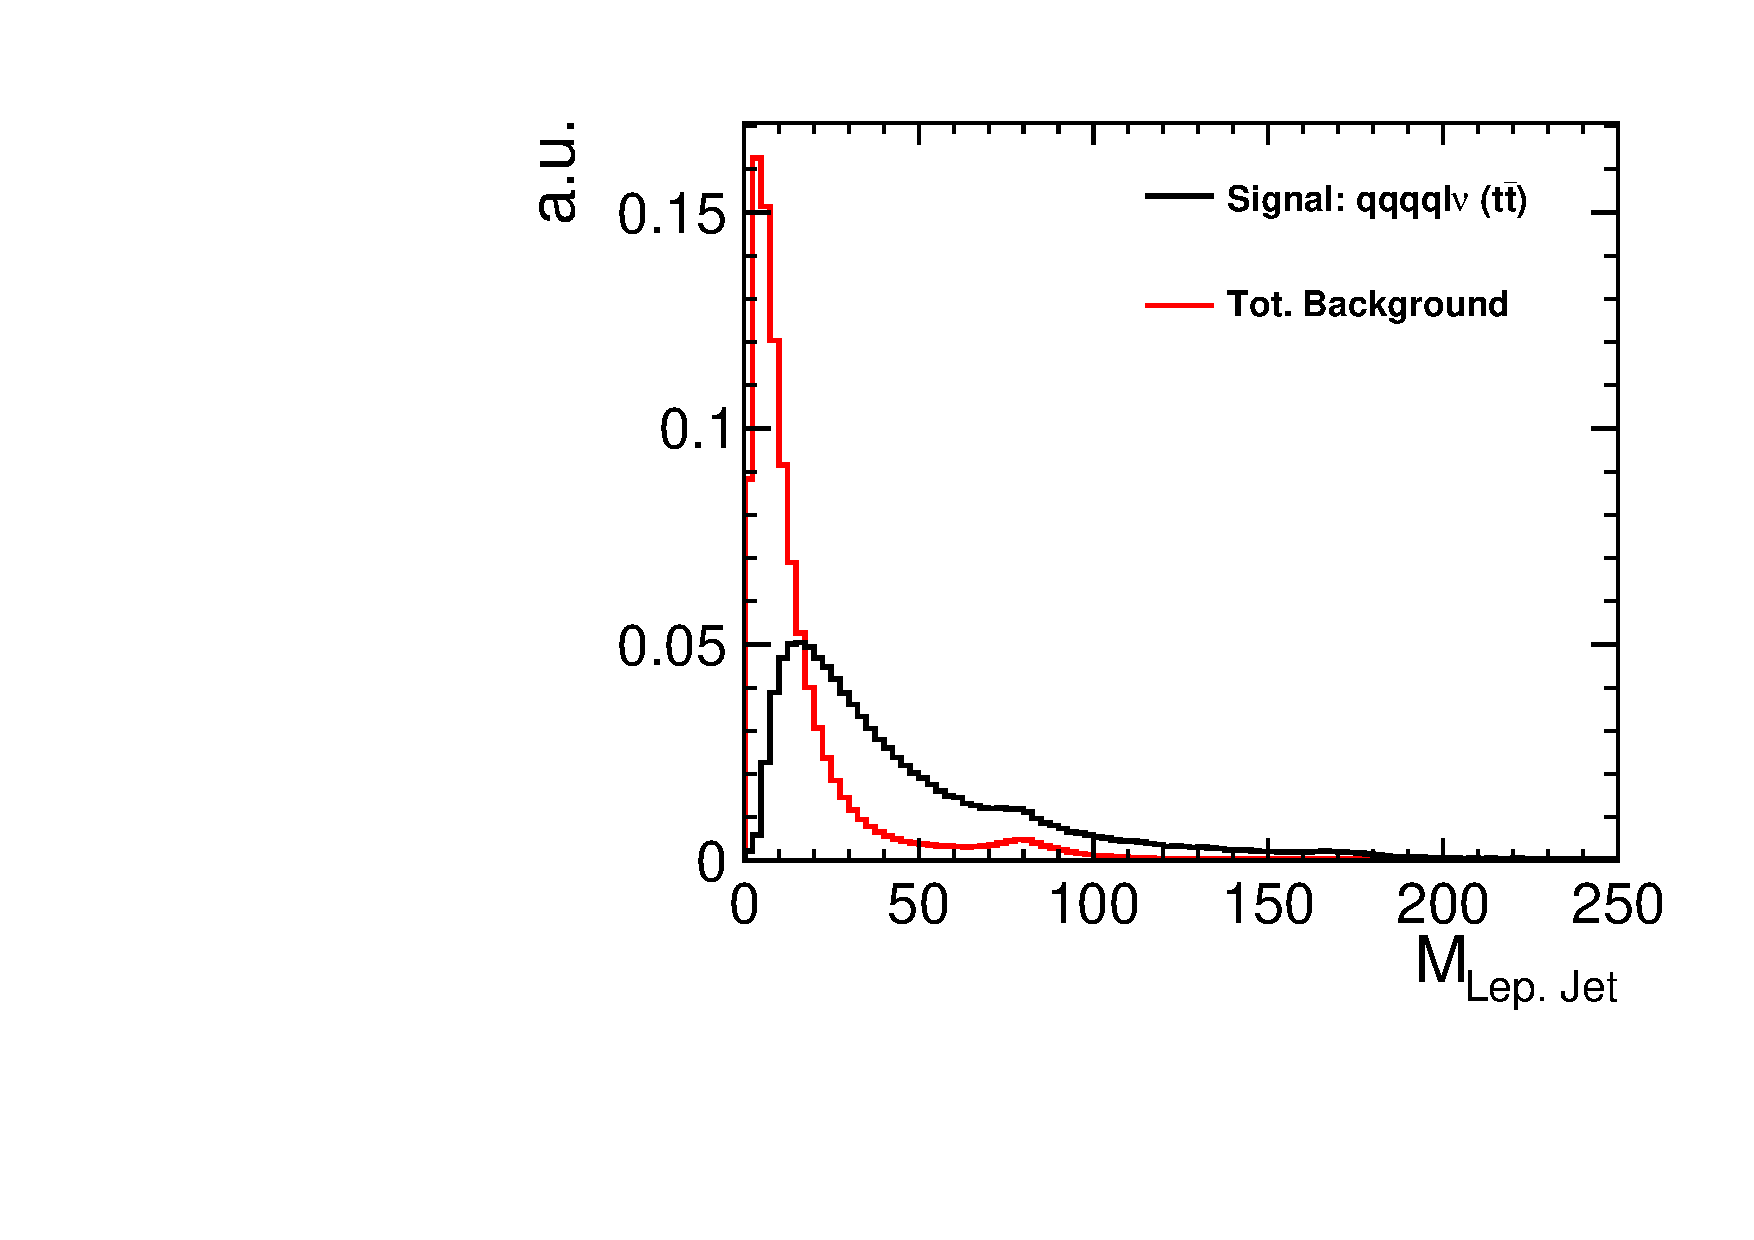
\includegraphics[width=0.75\linewidth]{TopAnalysis/figures/BDTVariables/LeptonicJetMass.pdf} 
    \caption{Mass of leptonic fat jet} 
    \vspace{4ex}
  \end{subfigure}
  \begin{subfigure}[b]{0.5\linewidth}
    \centering
    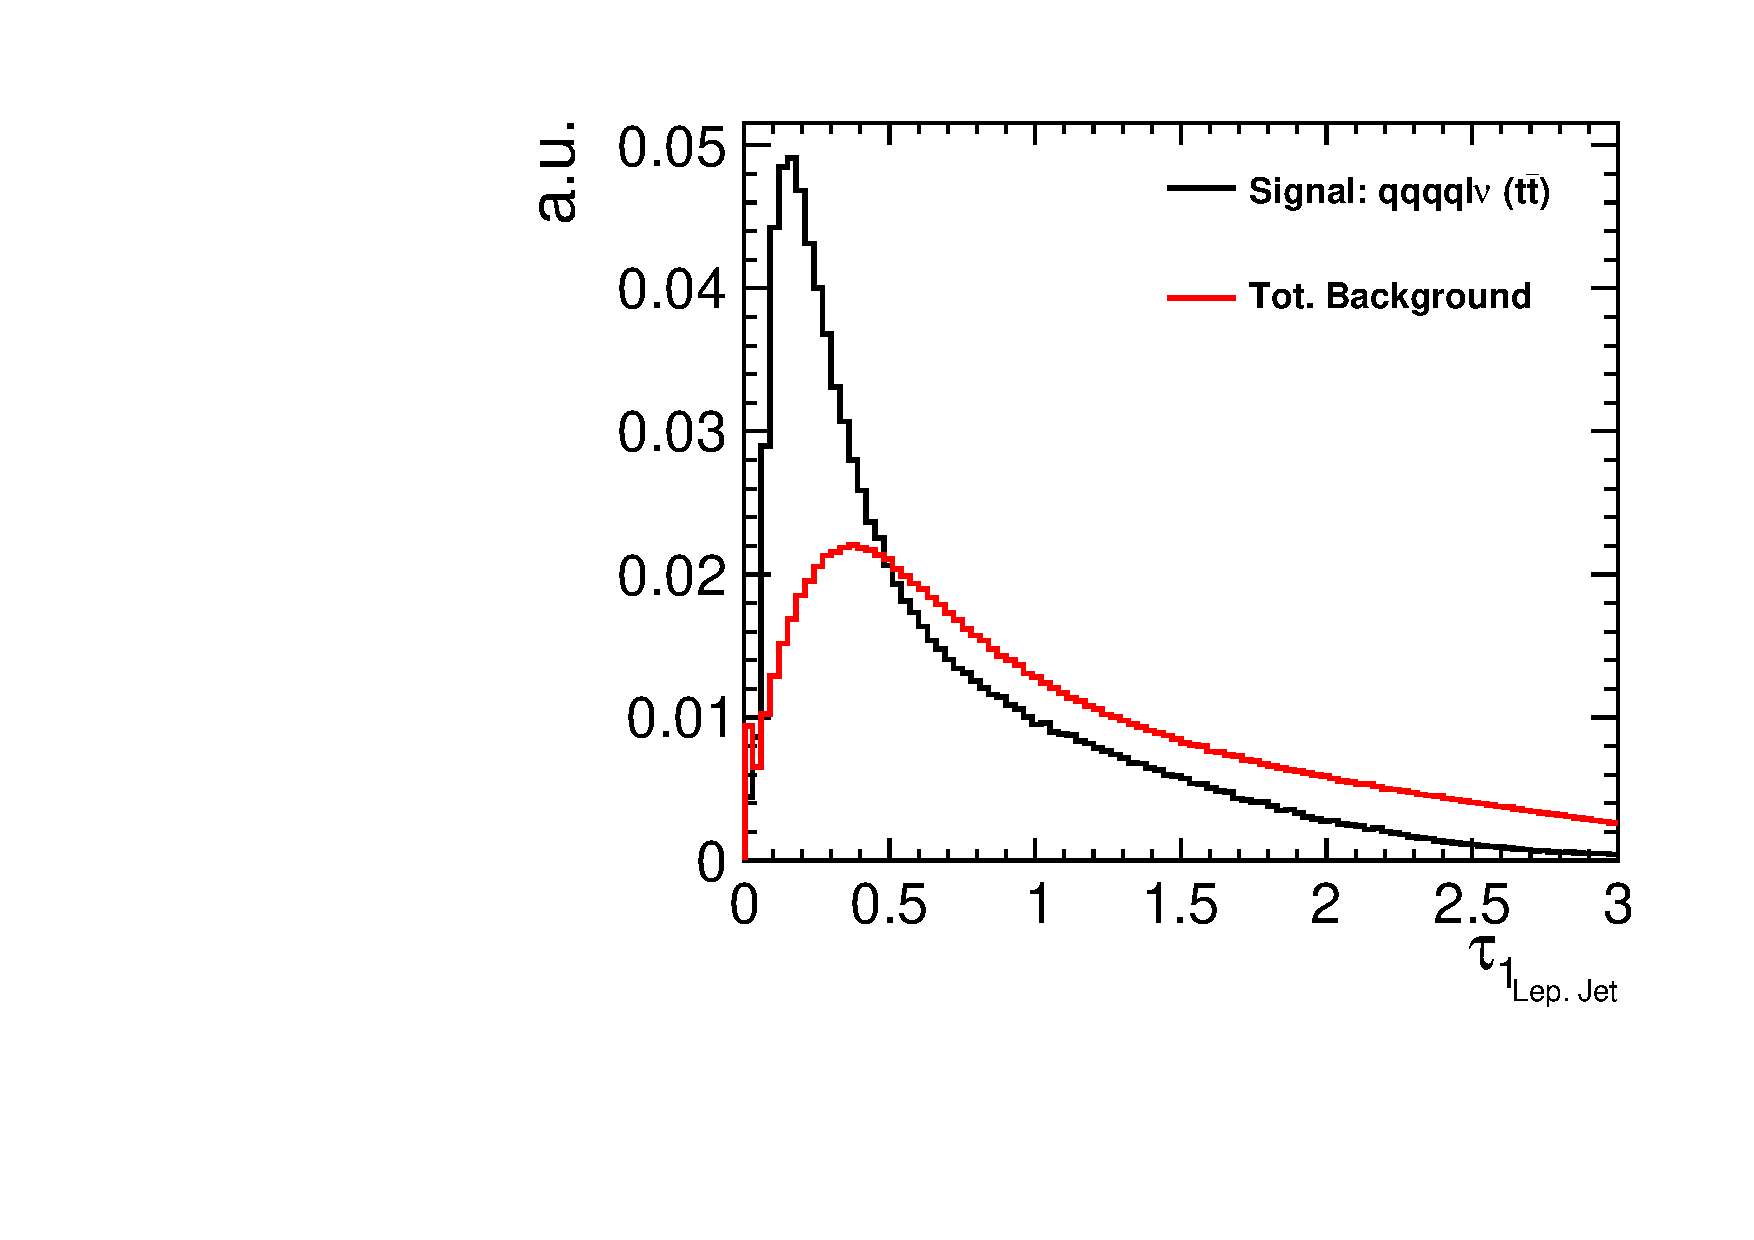
\includegraphics[width=0.75\linewidth]{TopAnalysis/figures/BDTVariables/Leptonic1SubJettiness.pdf} 
    \caption{Leptonic fat jet $\tau_1$} 
    \vspace{4ex}
  \end{subfigure}%%
  \begin{subfigure}[b]{0.5\linewidth}
    \centering
    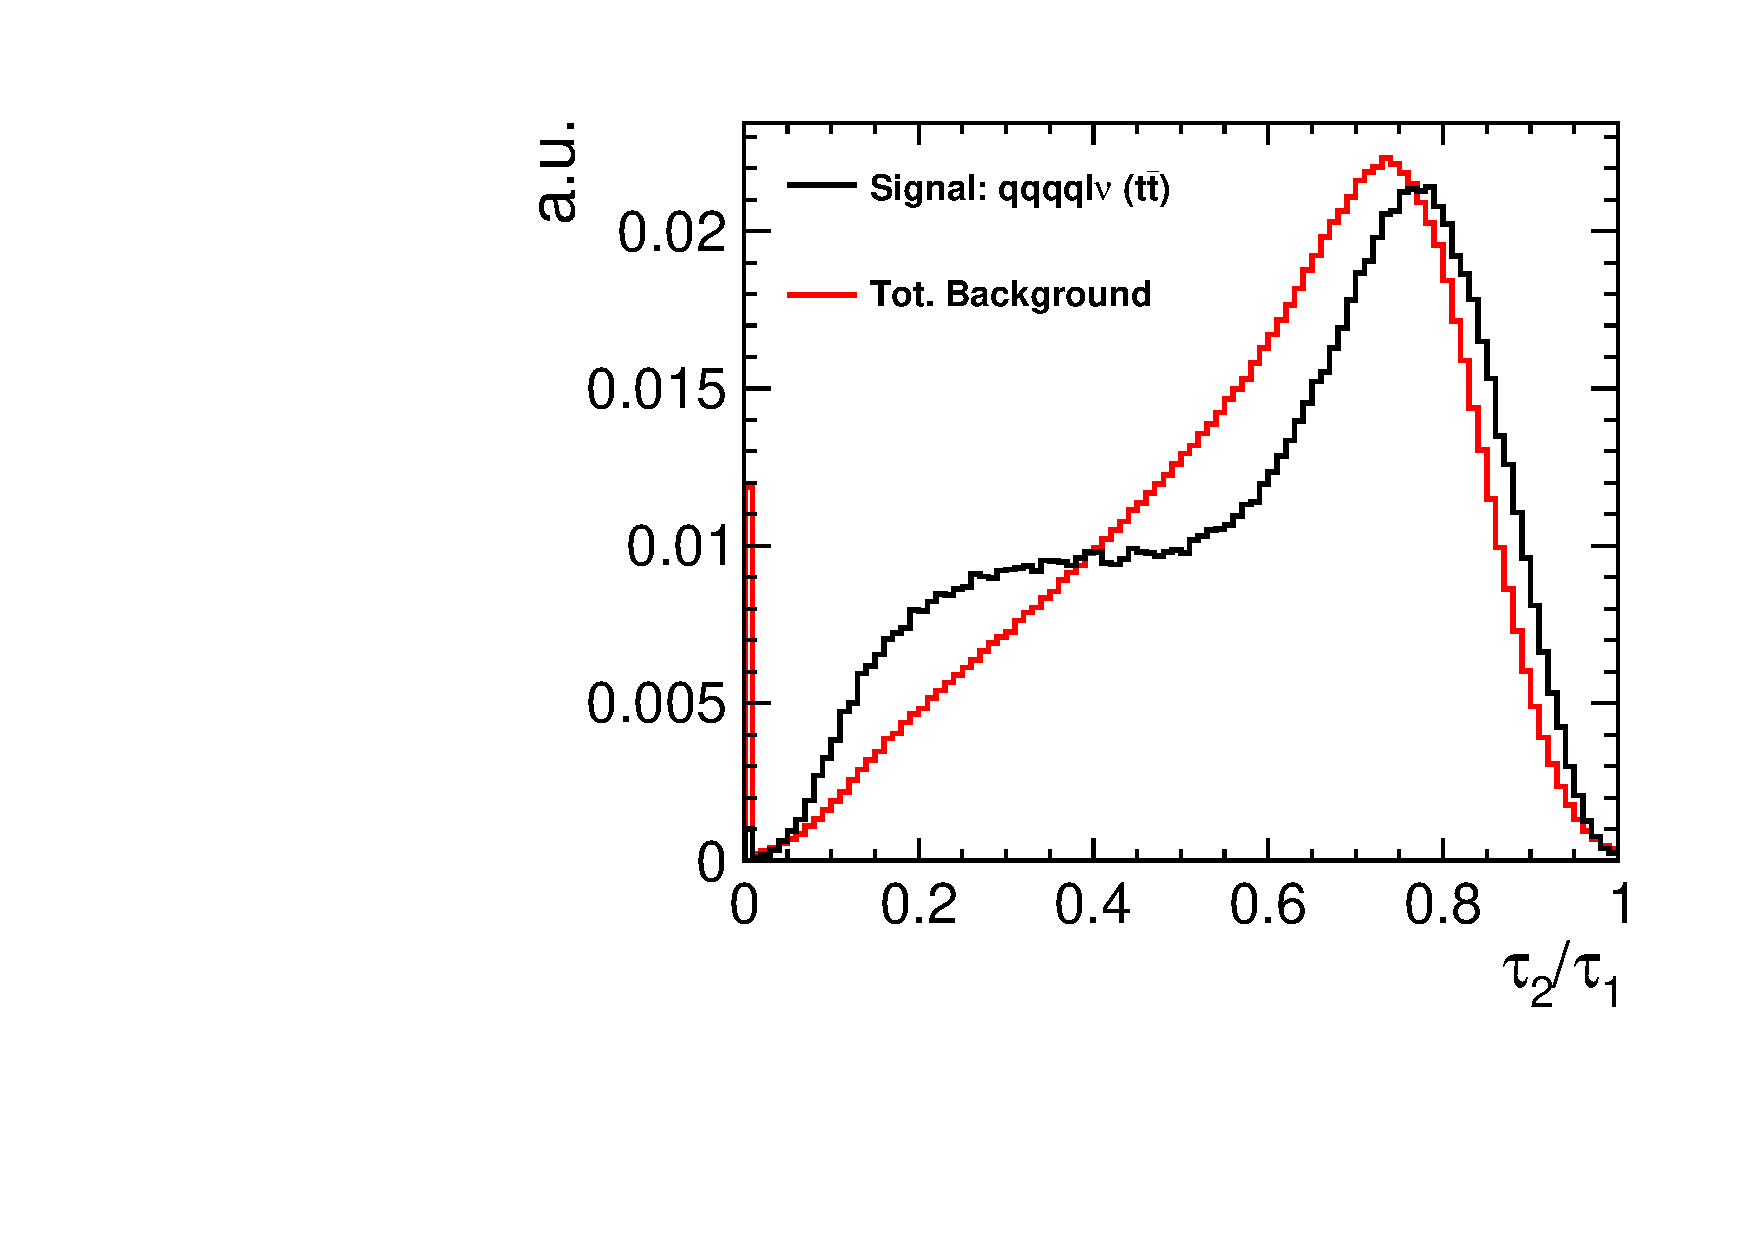
\includegraphics[width=0.75\linewidth]{TopAnalysis/figures/BDTVariables/Leptonic12Ratio.pdf} 
    \caption{Leptonic fat jet $\tau_2/\tau_1$} 
    \vspace{4ex}
  \end{subfigure}
\end{figure}

\begin{figure}[]\ContinuedFloat 
  \begin{subfigure}[b]{0.5\linewidth}
    \centering
    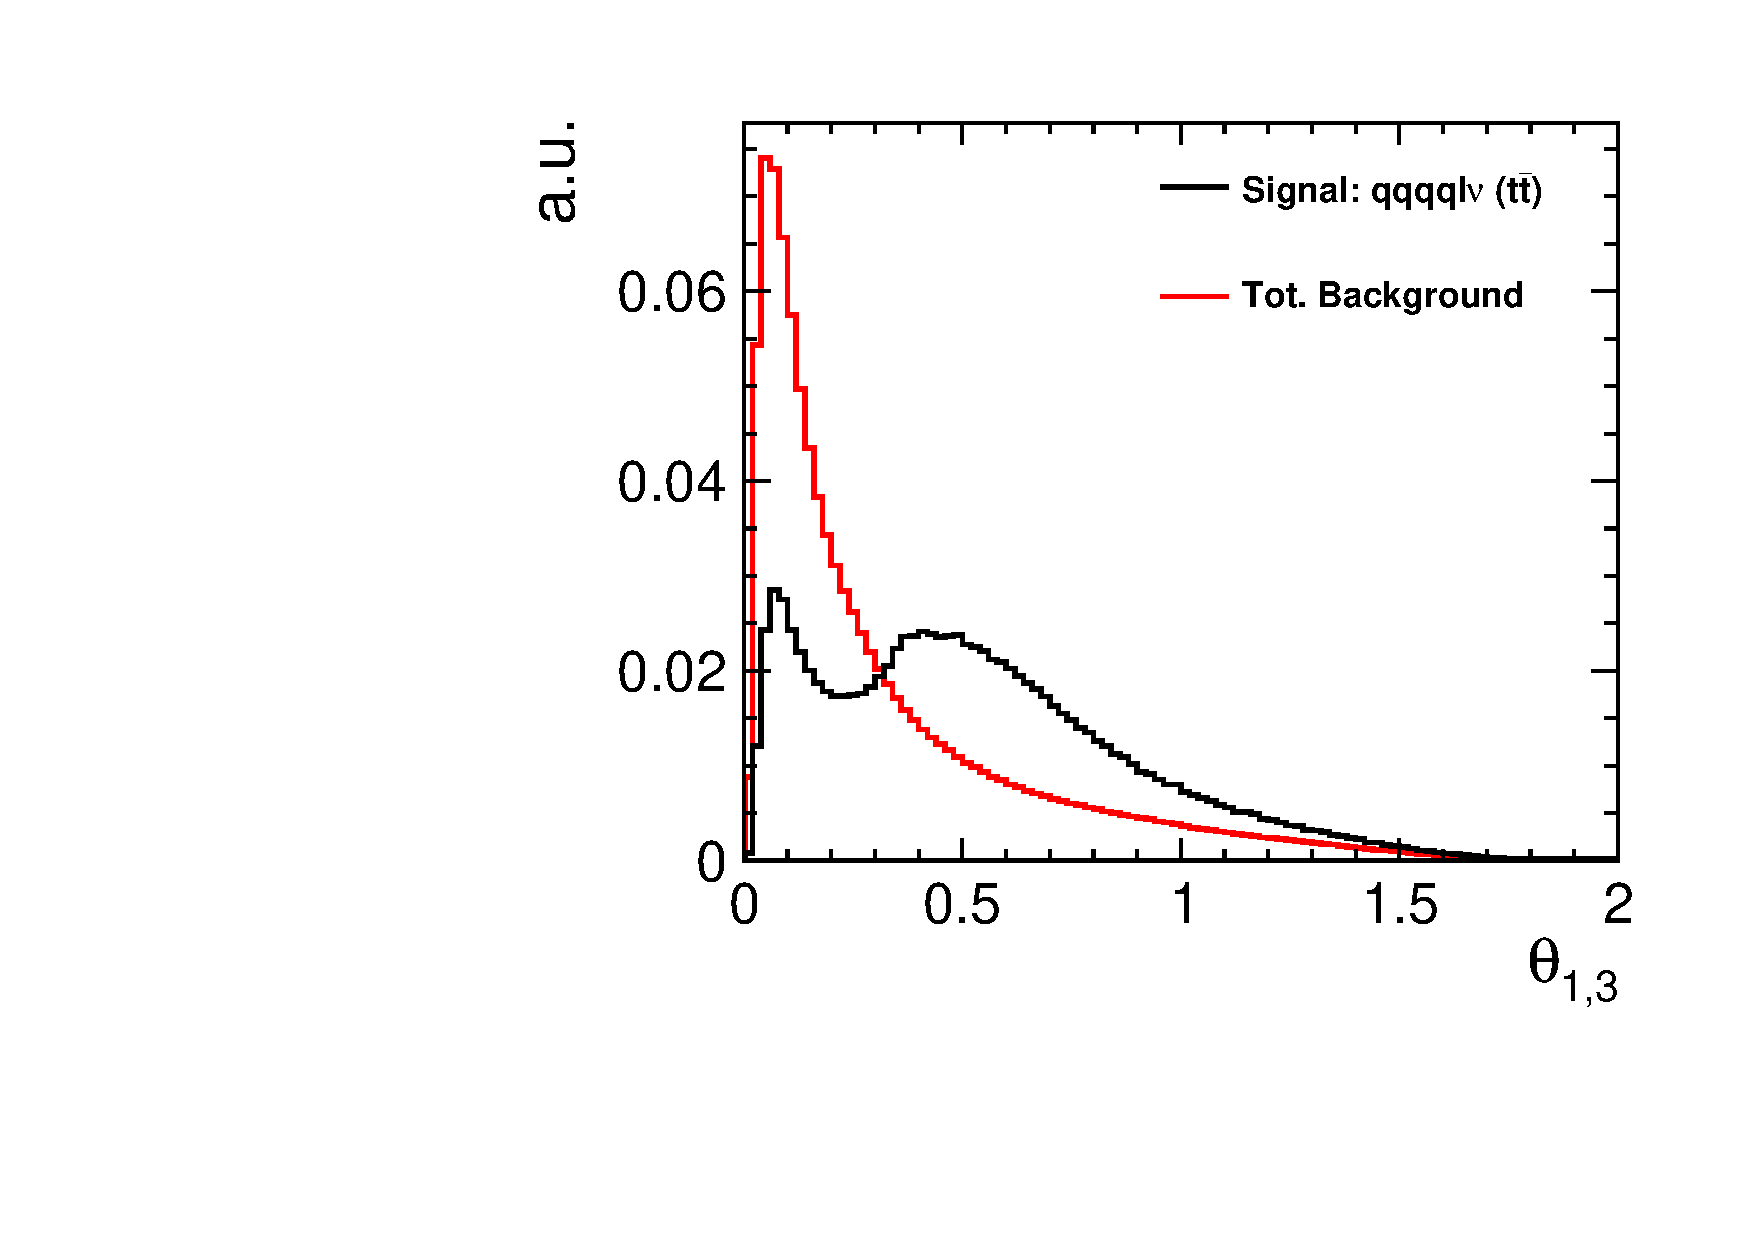
\includegraphics[width=0.75\linewidth]{TopAnalysis/figures/BDTVariables/HighEtoLowEDira.pdf} 
    \caption{$\theta_{1,3}$} 
    \vspace{4ex}
  \end{subfigure}%% 
  \begin{subfigure}[b]{0.5\linewidth}
    \centering
    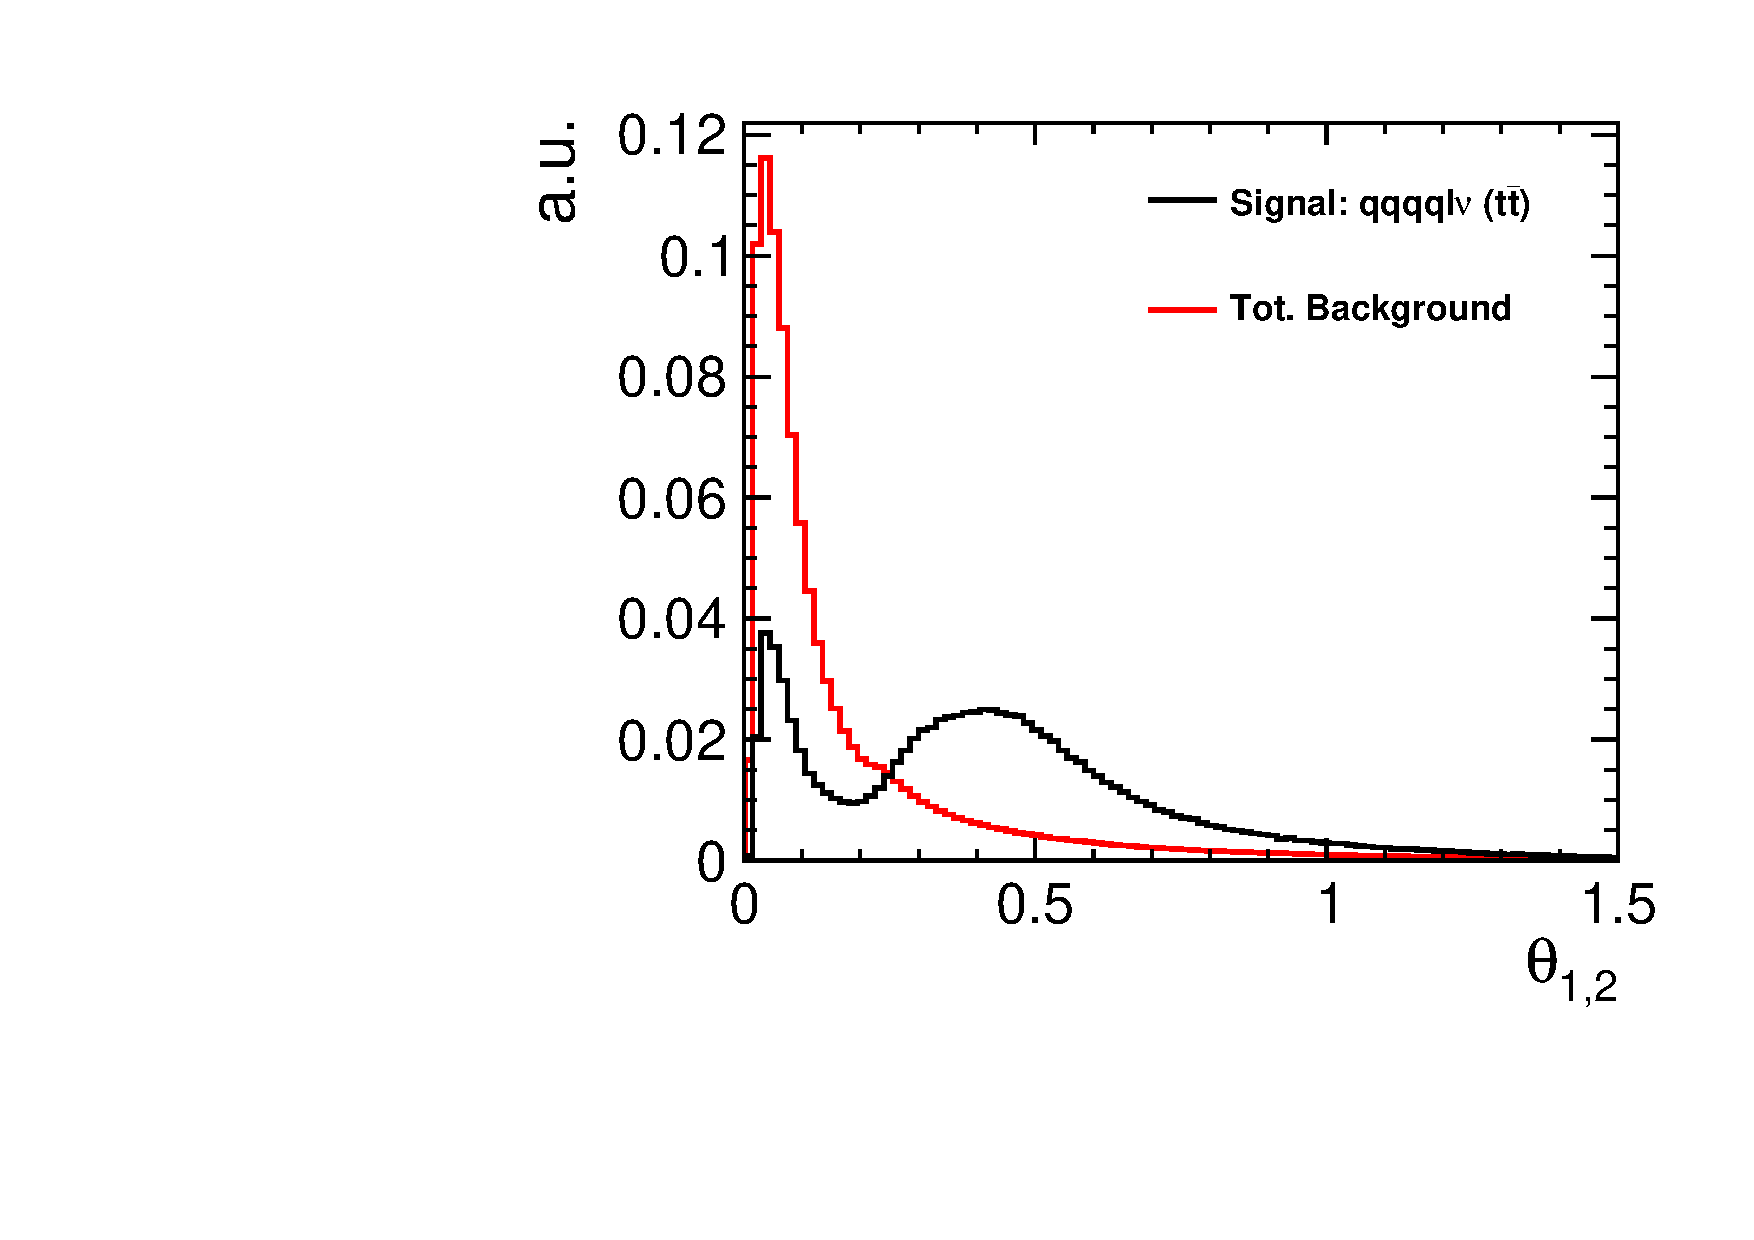
\includegraphics[width=0.75\linewidth]{TopAnalysis/figures/BDTVariables/HighEtoMidEDira.pdf} 
    \caption{$\theta_{1,2}$} 
    \vspace{4ex}
  \end{subfigure} 
  \begin{subfigure}[b]{0.5\linewidth}
    \centering
    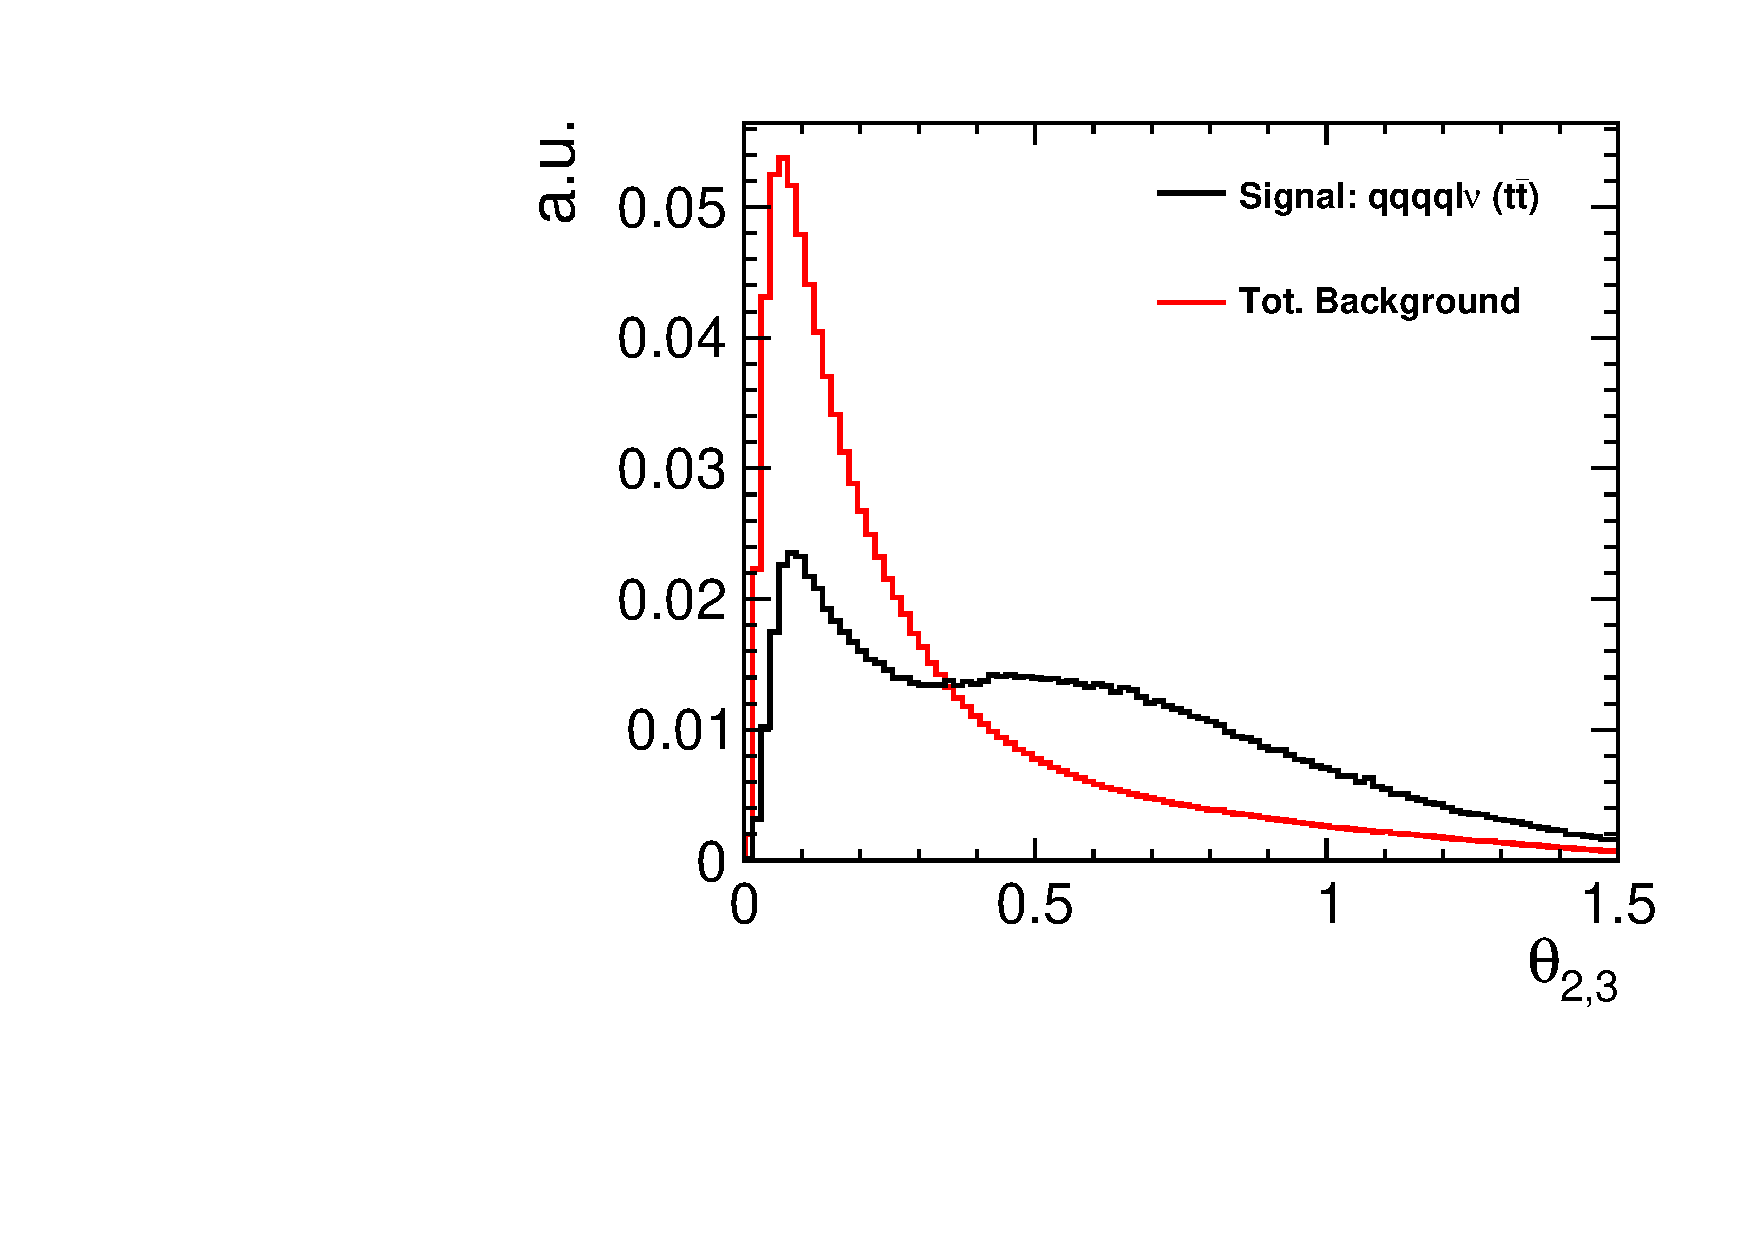
\includegraphics[width=0.75\linewidth]{TopAnalysis/figures/BDTVariables/MidEtoLowEDira.pdf} 
    \caption{$\theta_{2,3}$} 
    \vspace{4ex}
  \end{subfigure}%%
  \begin{subfigure}[b]{0.5\linewidth}
    \centering
    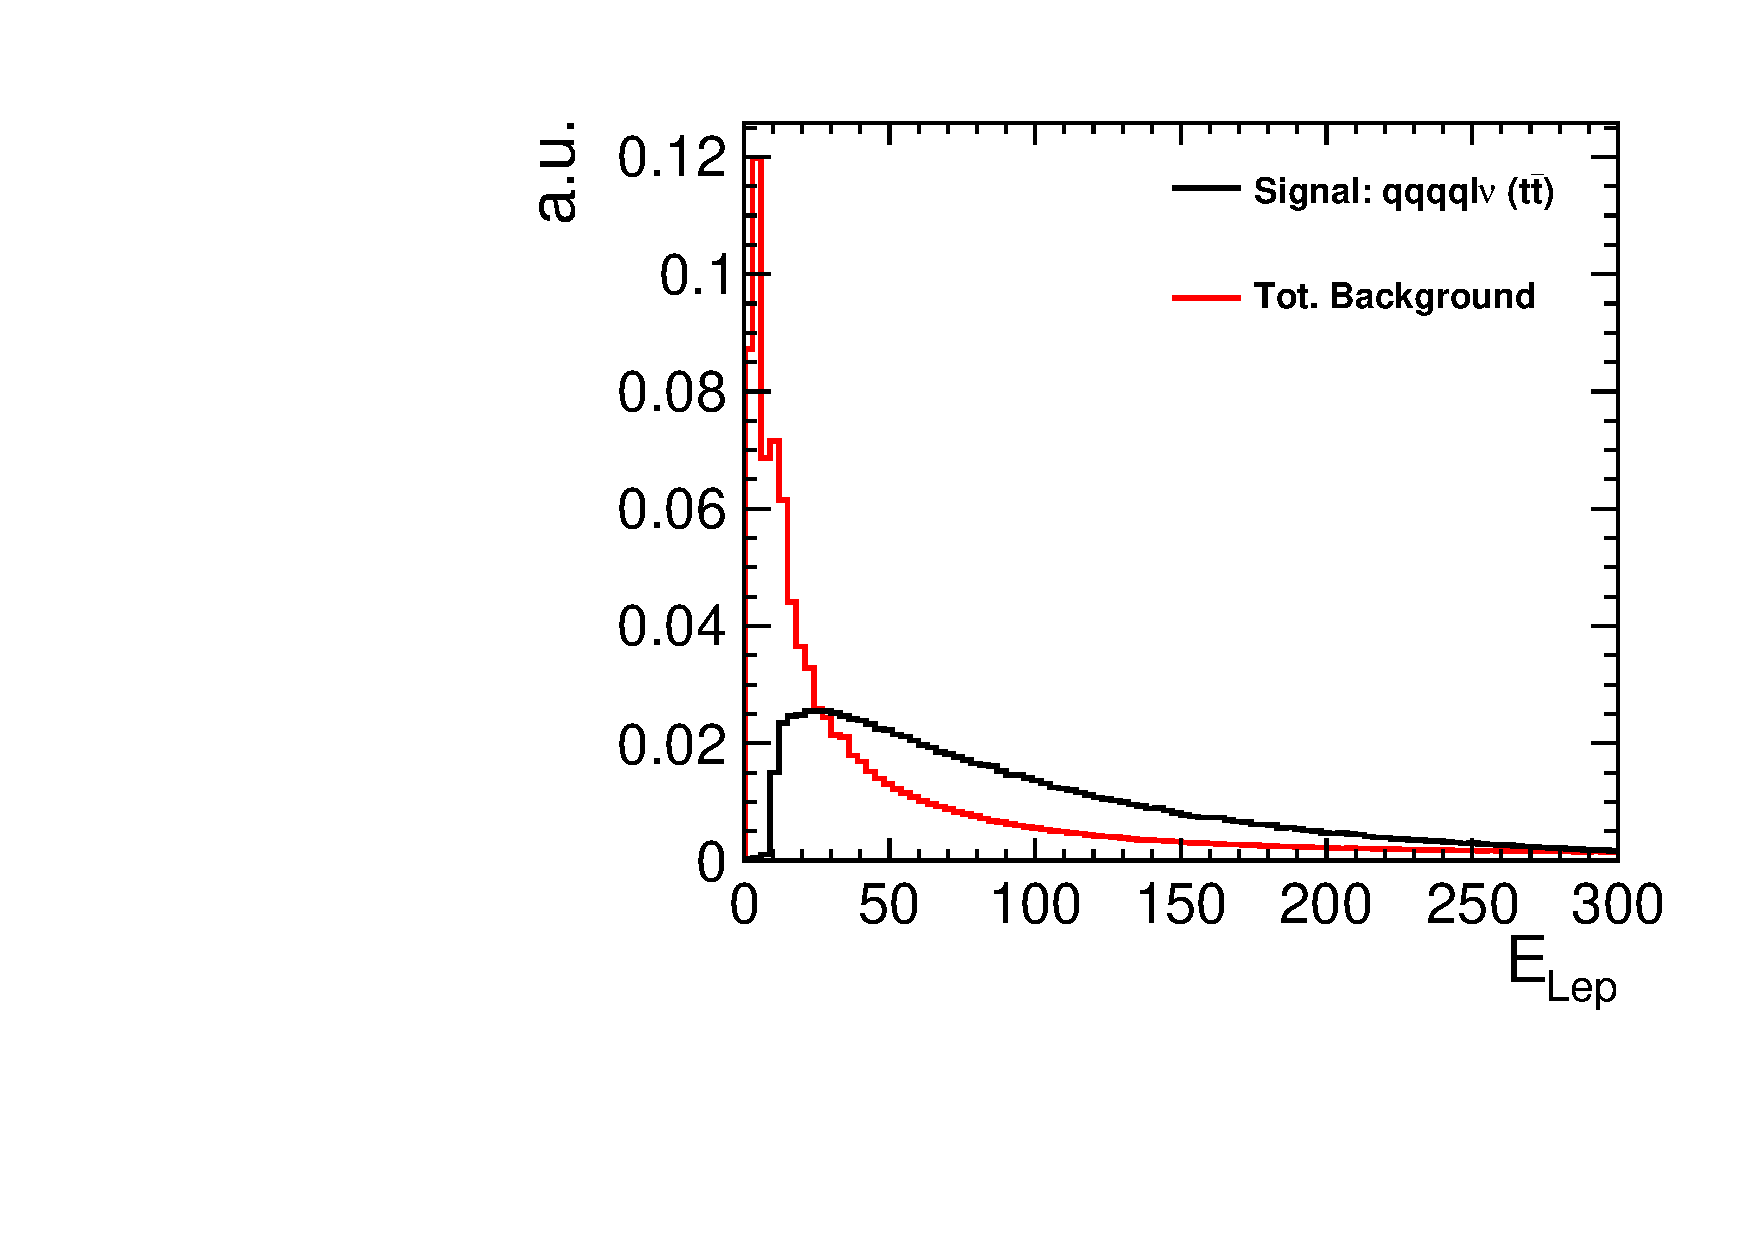
\includegraphics[width=0.75\linewidth]{TopAnalysis/figures/BDTVariables/IsoLepEnergy.pdf} 
    \caption{Lepton Energy} 
    \vspace{4ex}
  \end{subfigure}
  \begin{subfigure}[b]{0.5\linewidth}
    \centering
    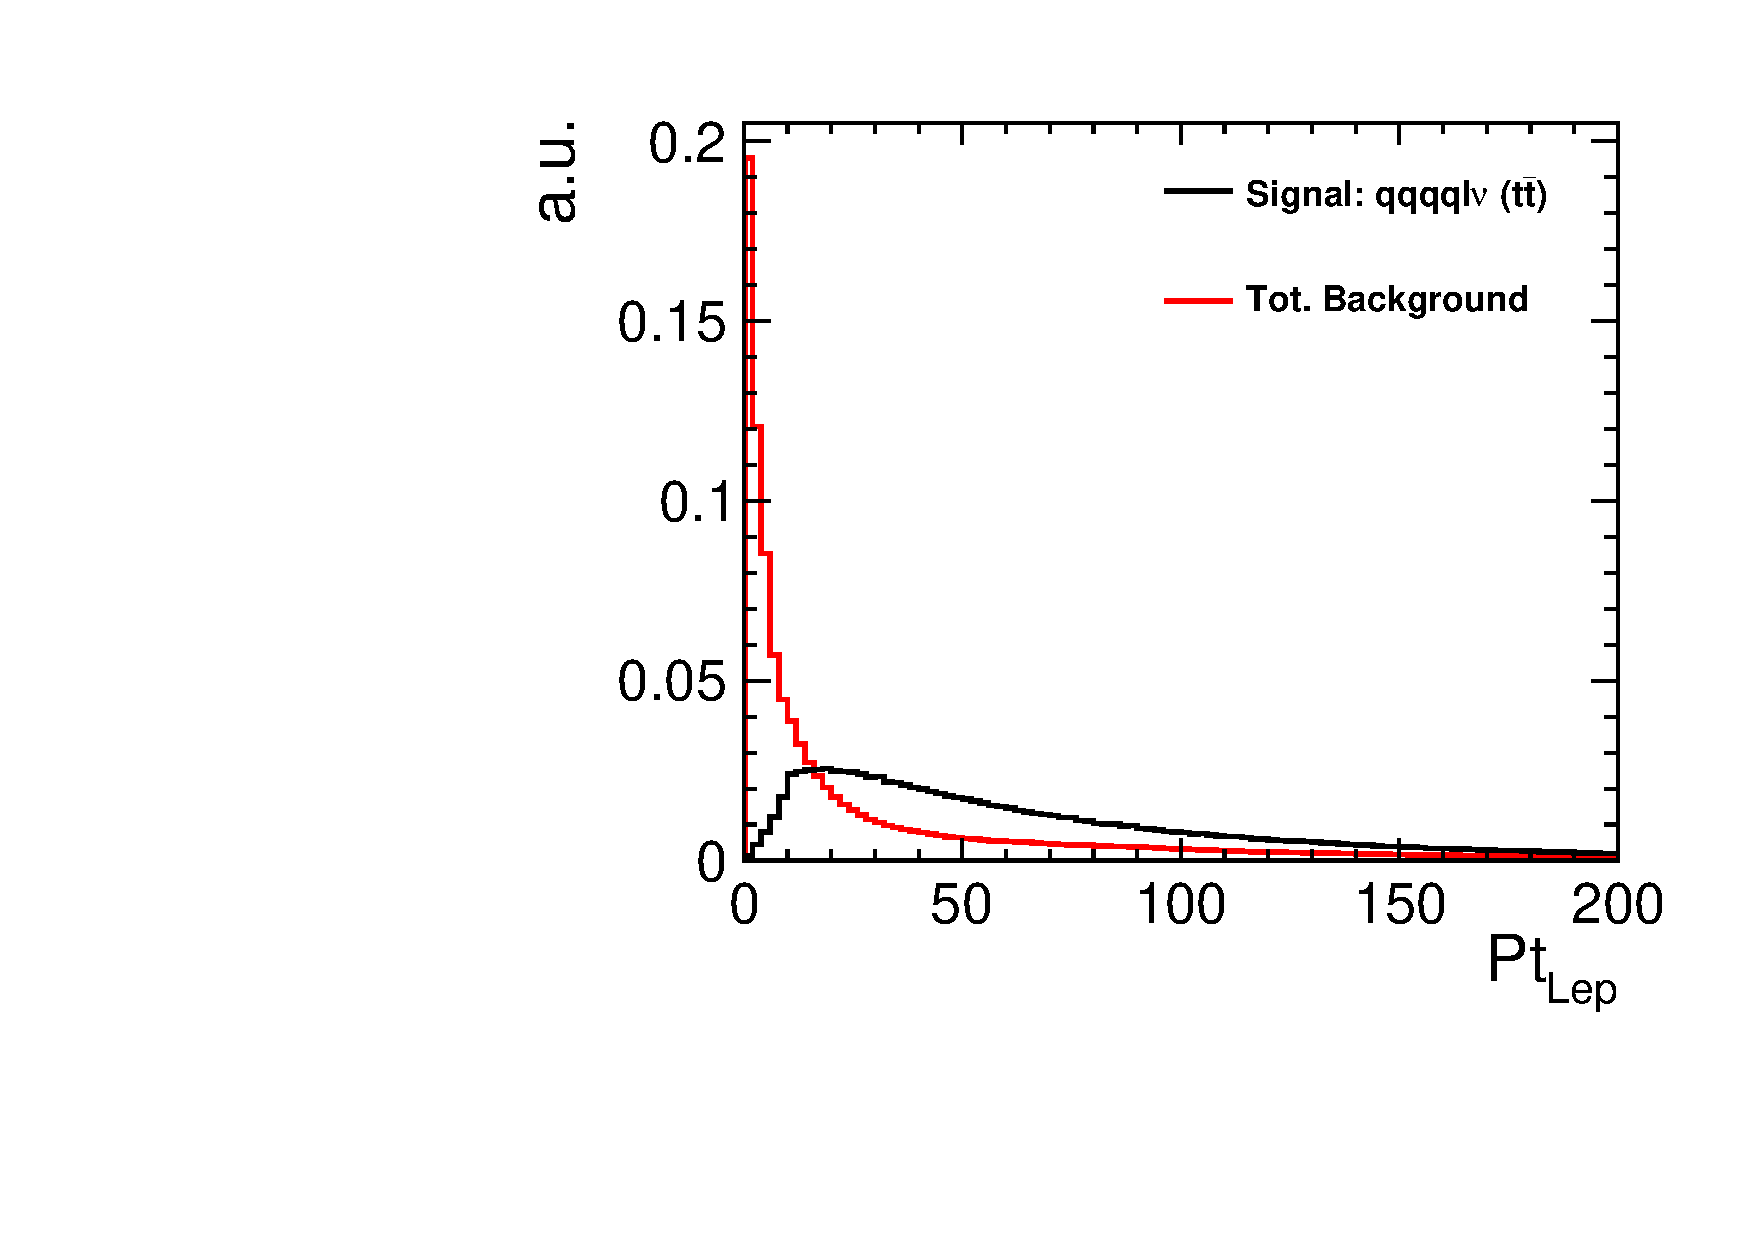
\includegraphics[width=0.75\linewidth]{TopAnalysis/figures/BDTVariables/IsoLepPt.pdf} 
    \caption{Lepton transverse momentum} 
    \vspace{4ex}
  \end{subfigure}%%
  \begin{subfigure}[b]{0.5\linewidth}
    \centering
    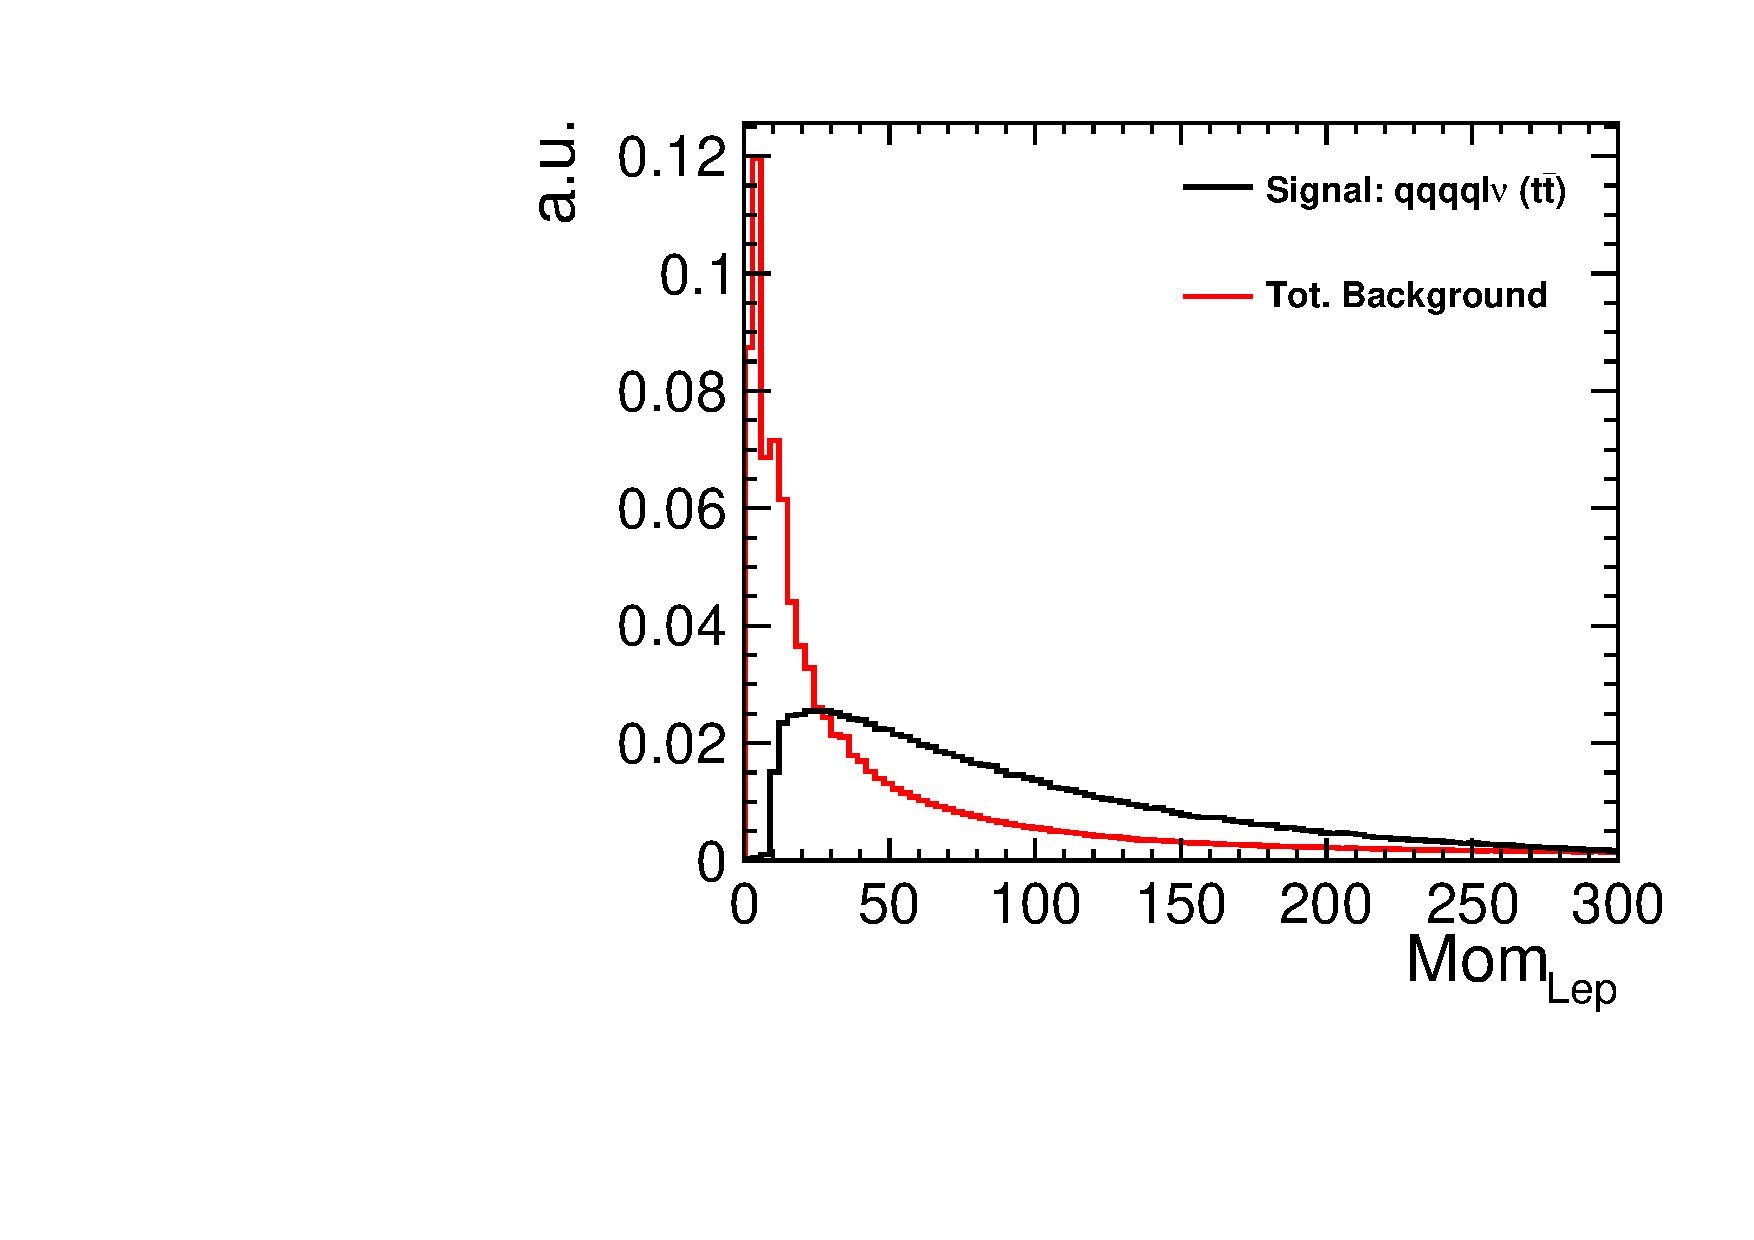
\includegraphics[width=0.75\linewidth]{TopAnalysis/figures/BDTVariables/IsoLepMomentum.pdf} 
    \caption{Lepton momentum} 
    \vspace{4ex}
  \end{subfigure}
\end{figure}

\begin{figure}[]\ContinuedFloat 
  \begin{subfigure}[b]{0.5\linewidth}
    \centering
    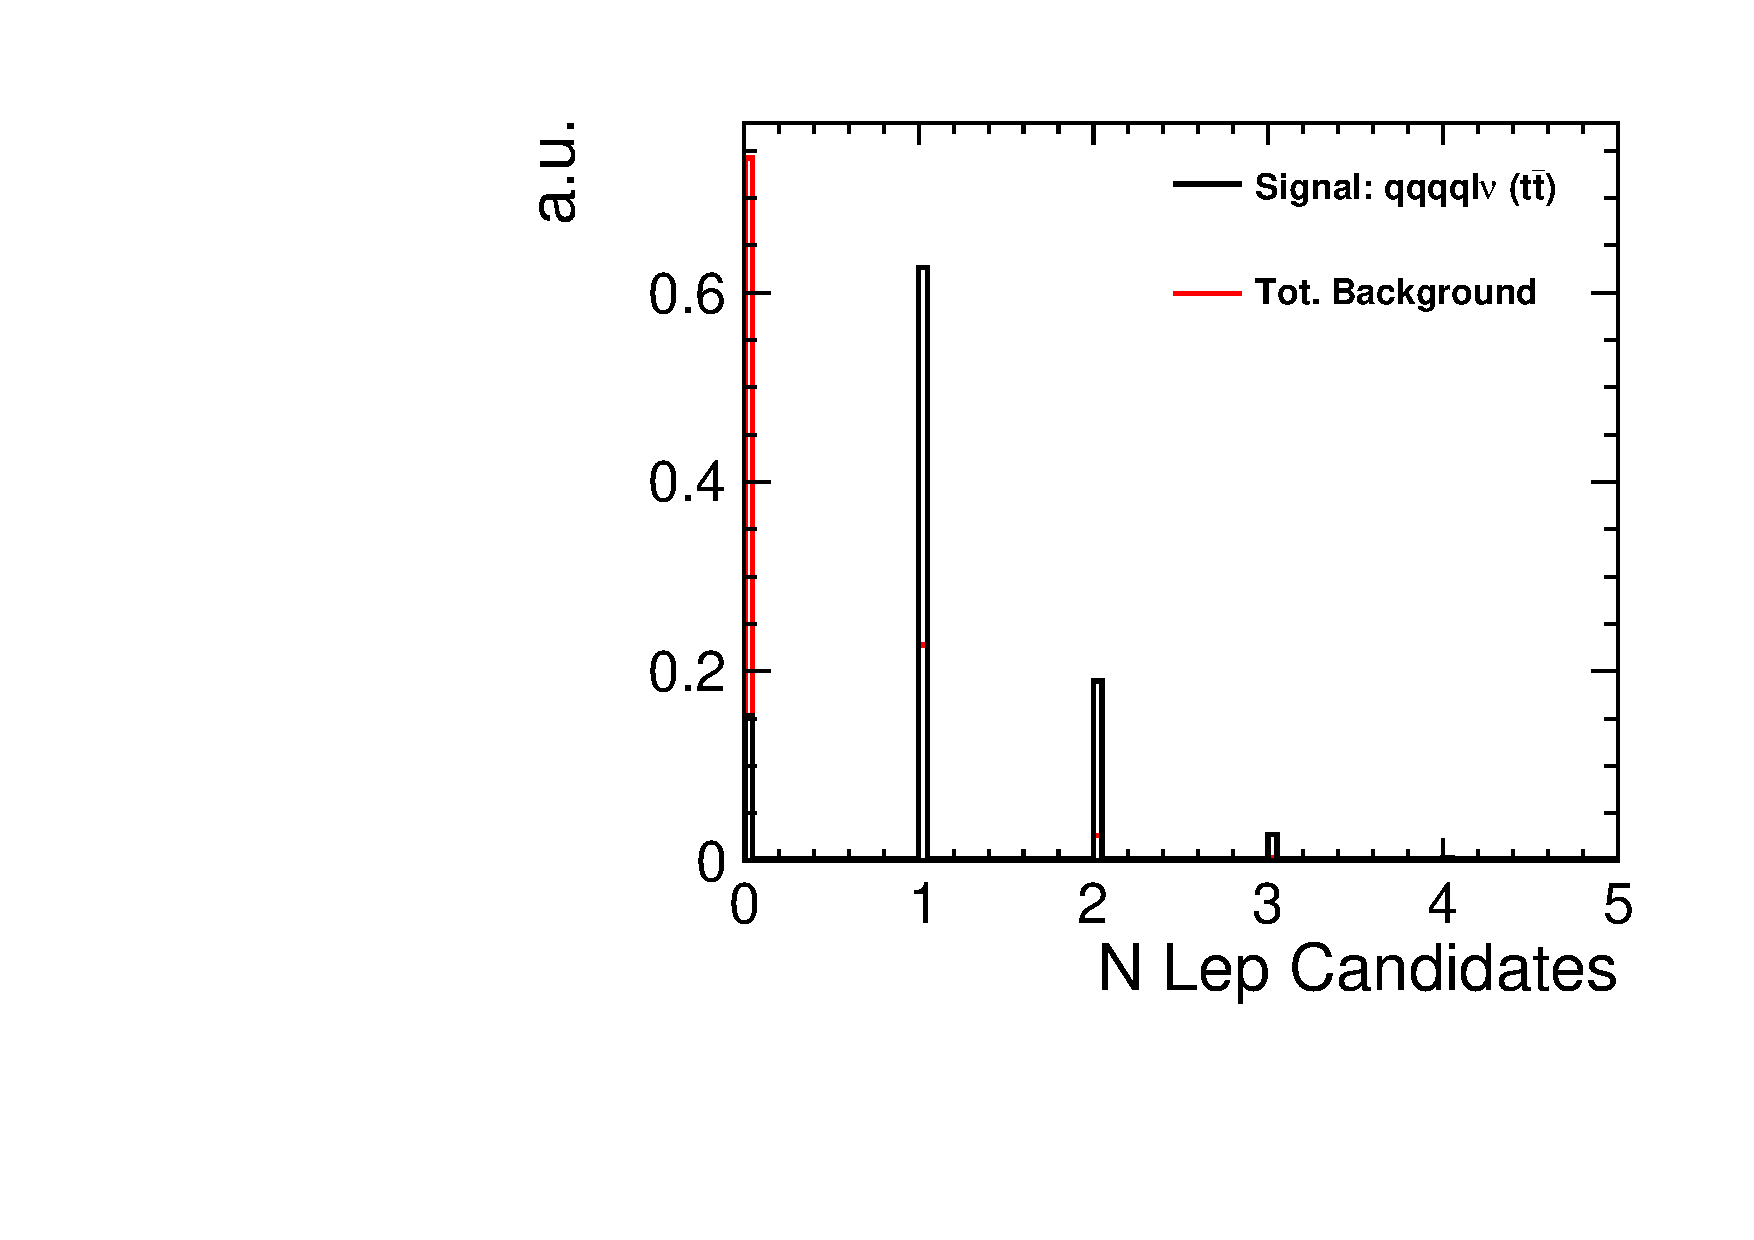
\includegraphics[width=0.75\linewidth]{TopAnalysis/figures/BDTVariables/NLeptonCandidates.pdf} 
    \caption{Number of lepton candidates with E$>$30 GeV } 
    \vspace{4ex}
  \end{subfigure}%% 
  \begin{subfigure}[b]{0.5\linewidth}
    \centering
    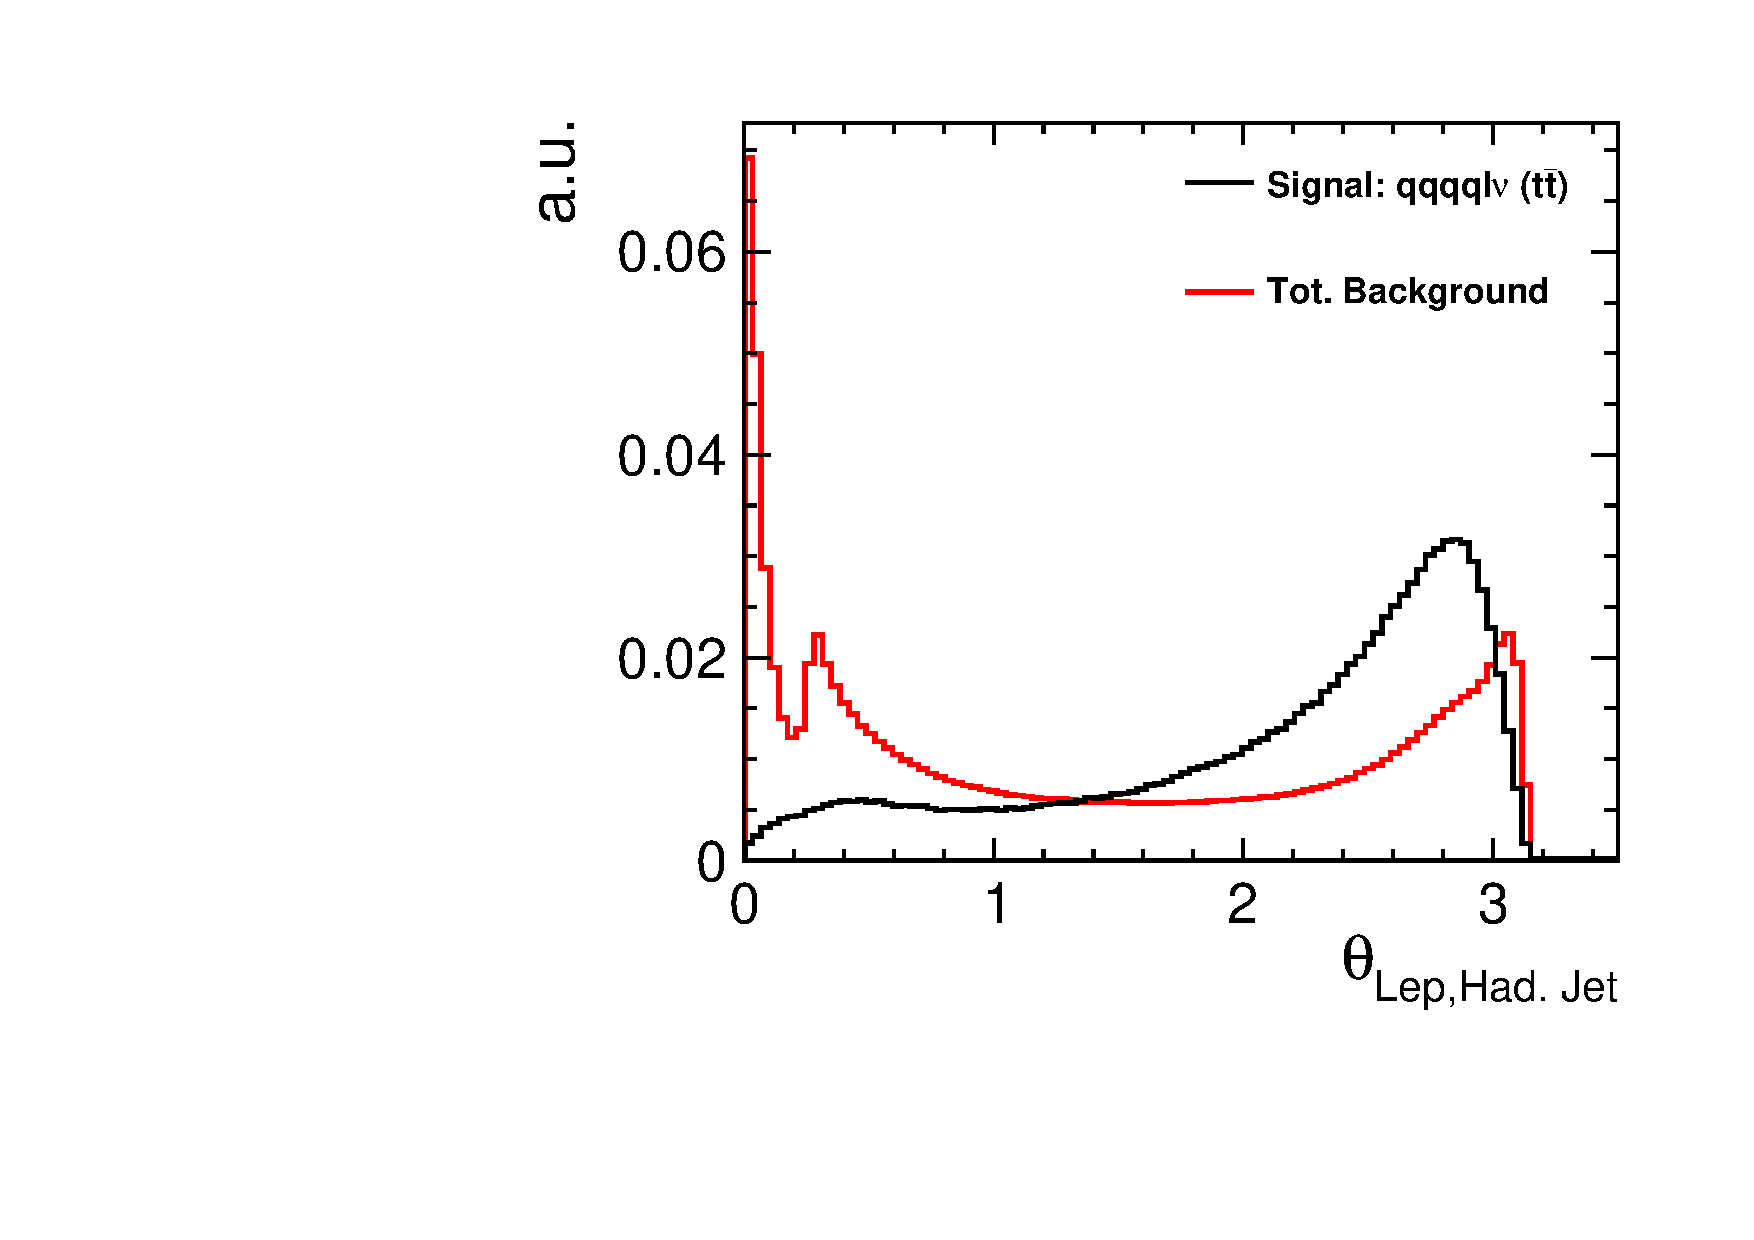
\includegraphics[width=0.75\linewidth]{TopAnalysis/figures/BDTVariables/TopLepDira.pdf} 
    \caption{Angular separation of the lepton and hadronic fat jet} 
    \vspace{4ex}
  \end{subfigure} 
  \begin{subfigure}[b]{0.5\linewidth}
    \centering
    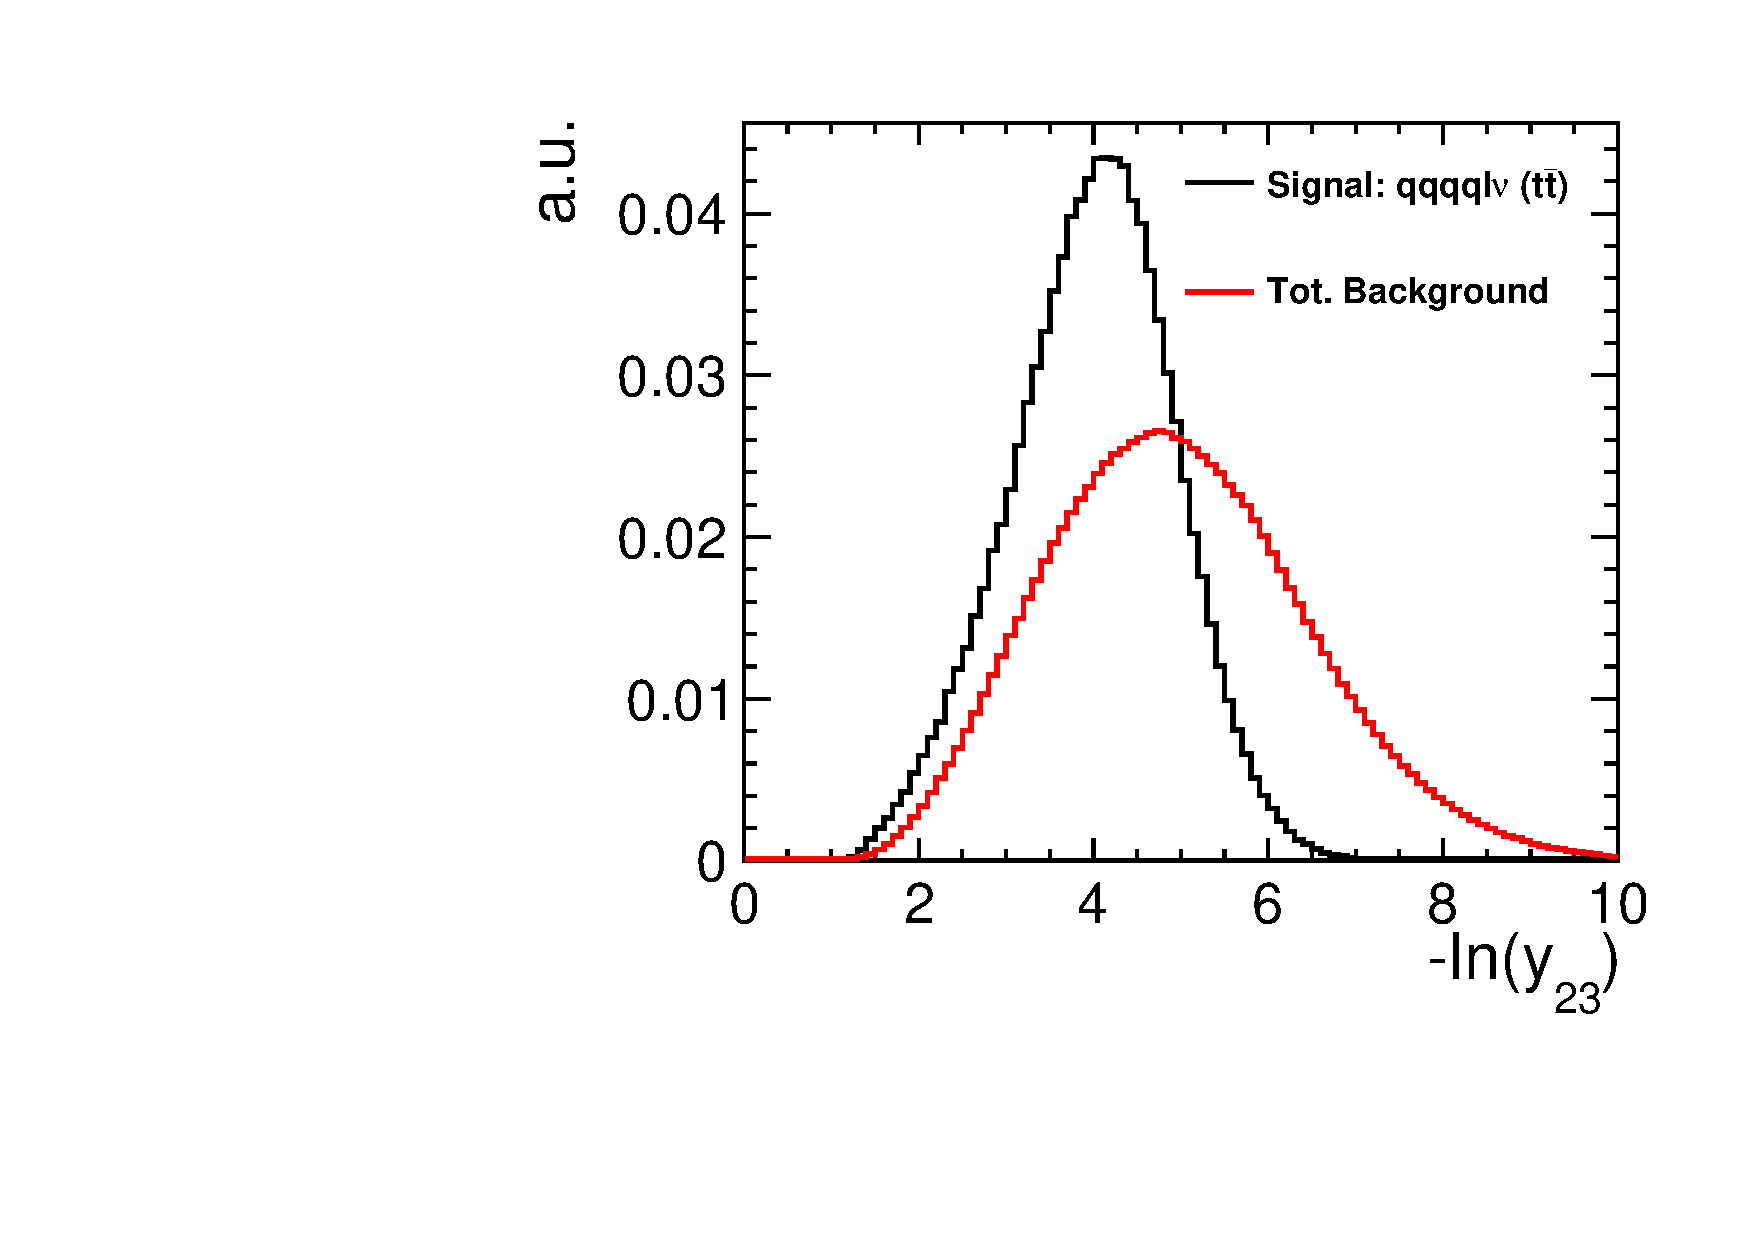
\includegraphics[width=0.75\linewidth]{TopAnalysis/figures/BDTVariables/Y23.pdf} 
    \caption{Jet resolution parameter $y_{23}$} 
    \vspace{4ex}
  \end{subfigure}%%
  \begin{subfigure}[b]{0.5\linewidth}
    \centering
    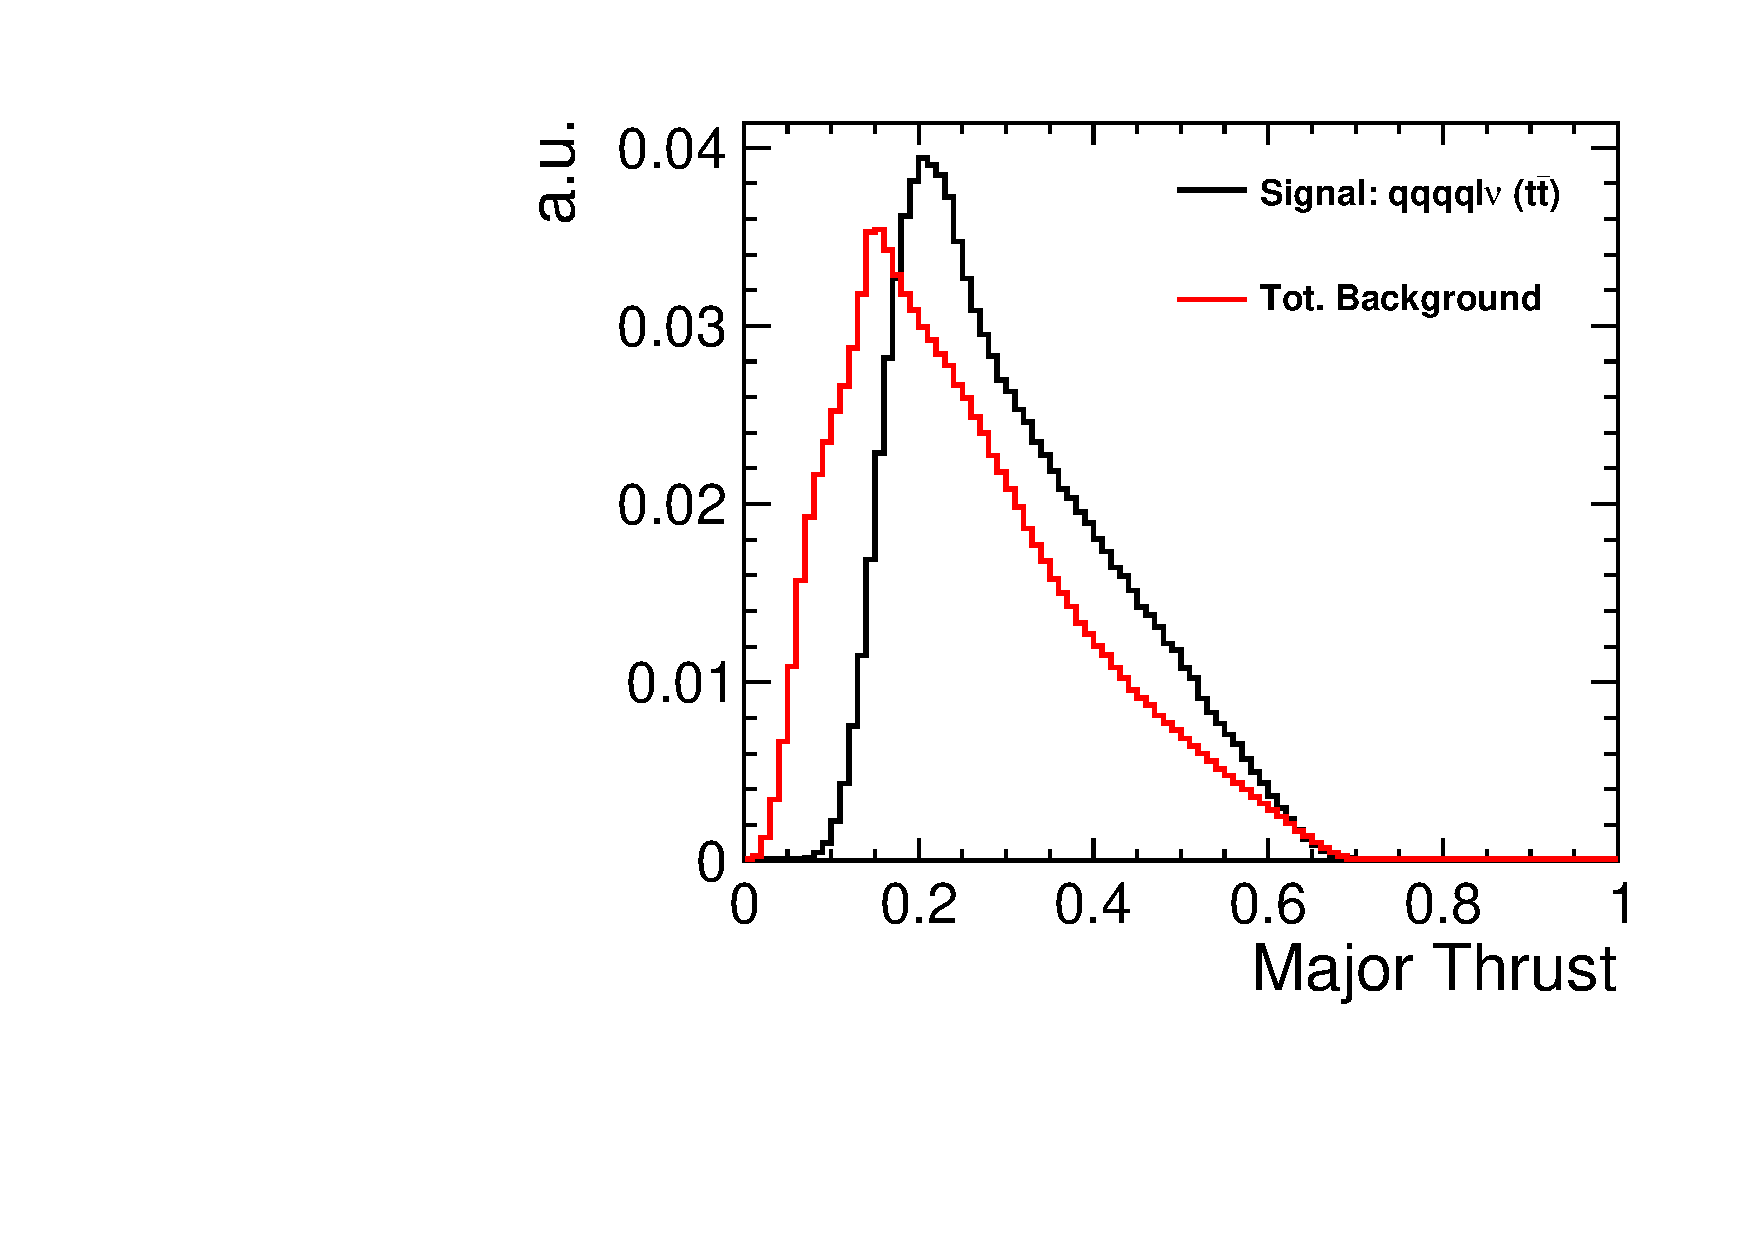
\includegraphics[width=0.75\linewidth]{TopAnalysis/figures/BDTVariables/majthval.pdf} 
    \caption{Major Thrust of event} 
    \vspace{4ex}
  \end{subfigure}
  \begin{subfigure}[b]{0.5\linewidth}
    \centering
    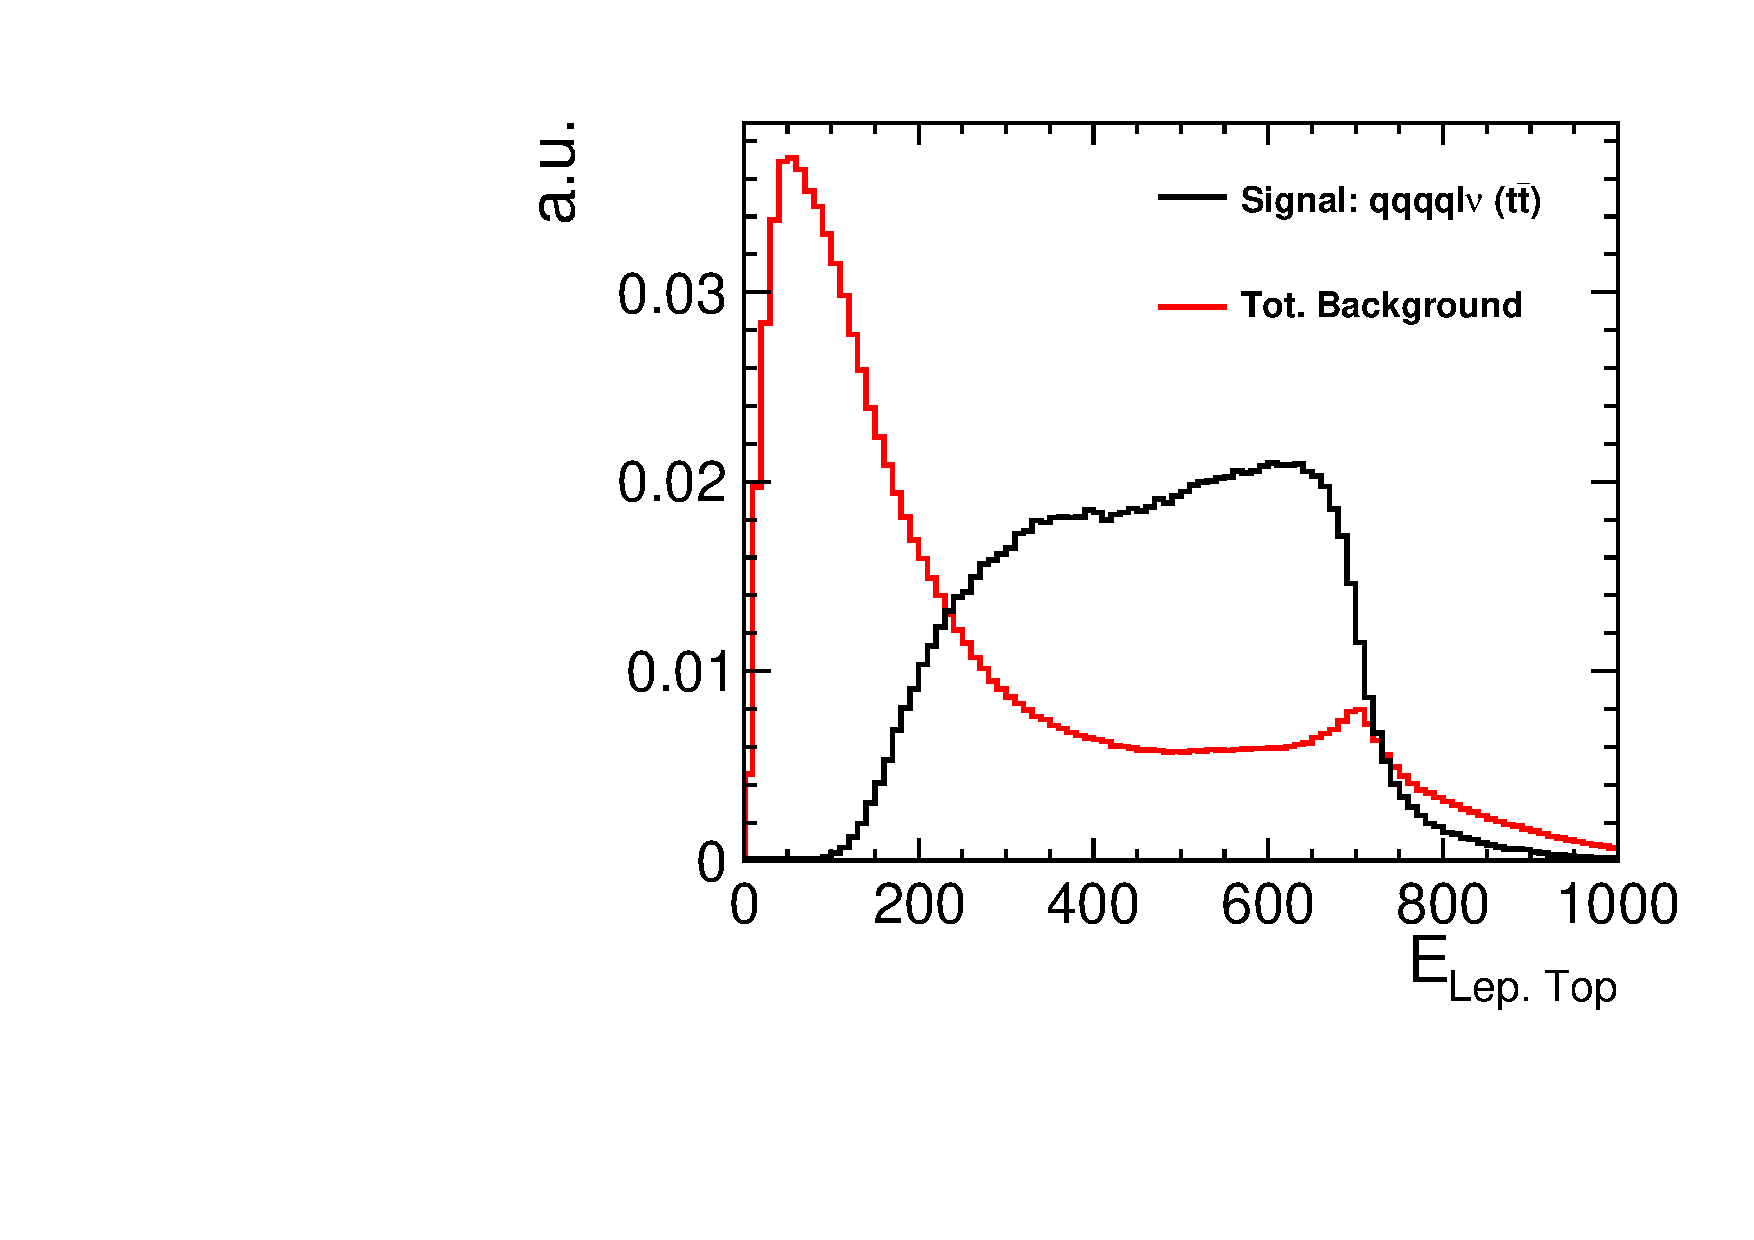
\includegraphics[width=0.75\linewidth]{TopAnalysis/figures/BDTVariables/LeptonicTopEnergy.pdf} 
    \caption{Energy of the leptonically decaying topx} 
    \vspace{4ex}
  \end{subfigure}%%
    \begin{subfigure}[b]{0.5\linewidth}
    \centering
    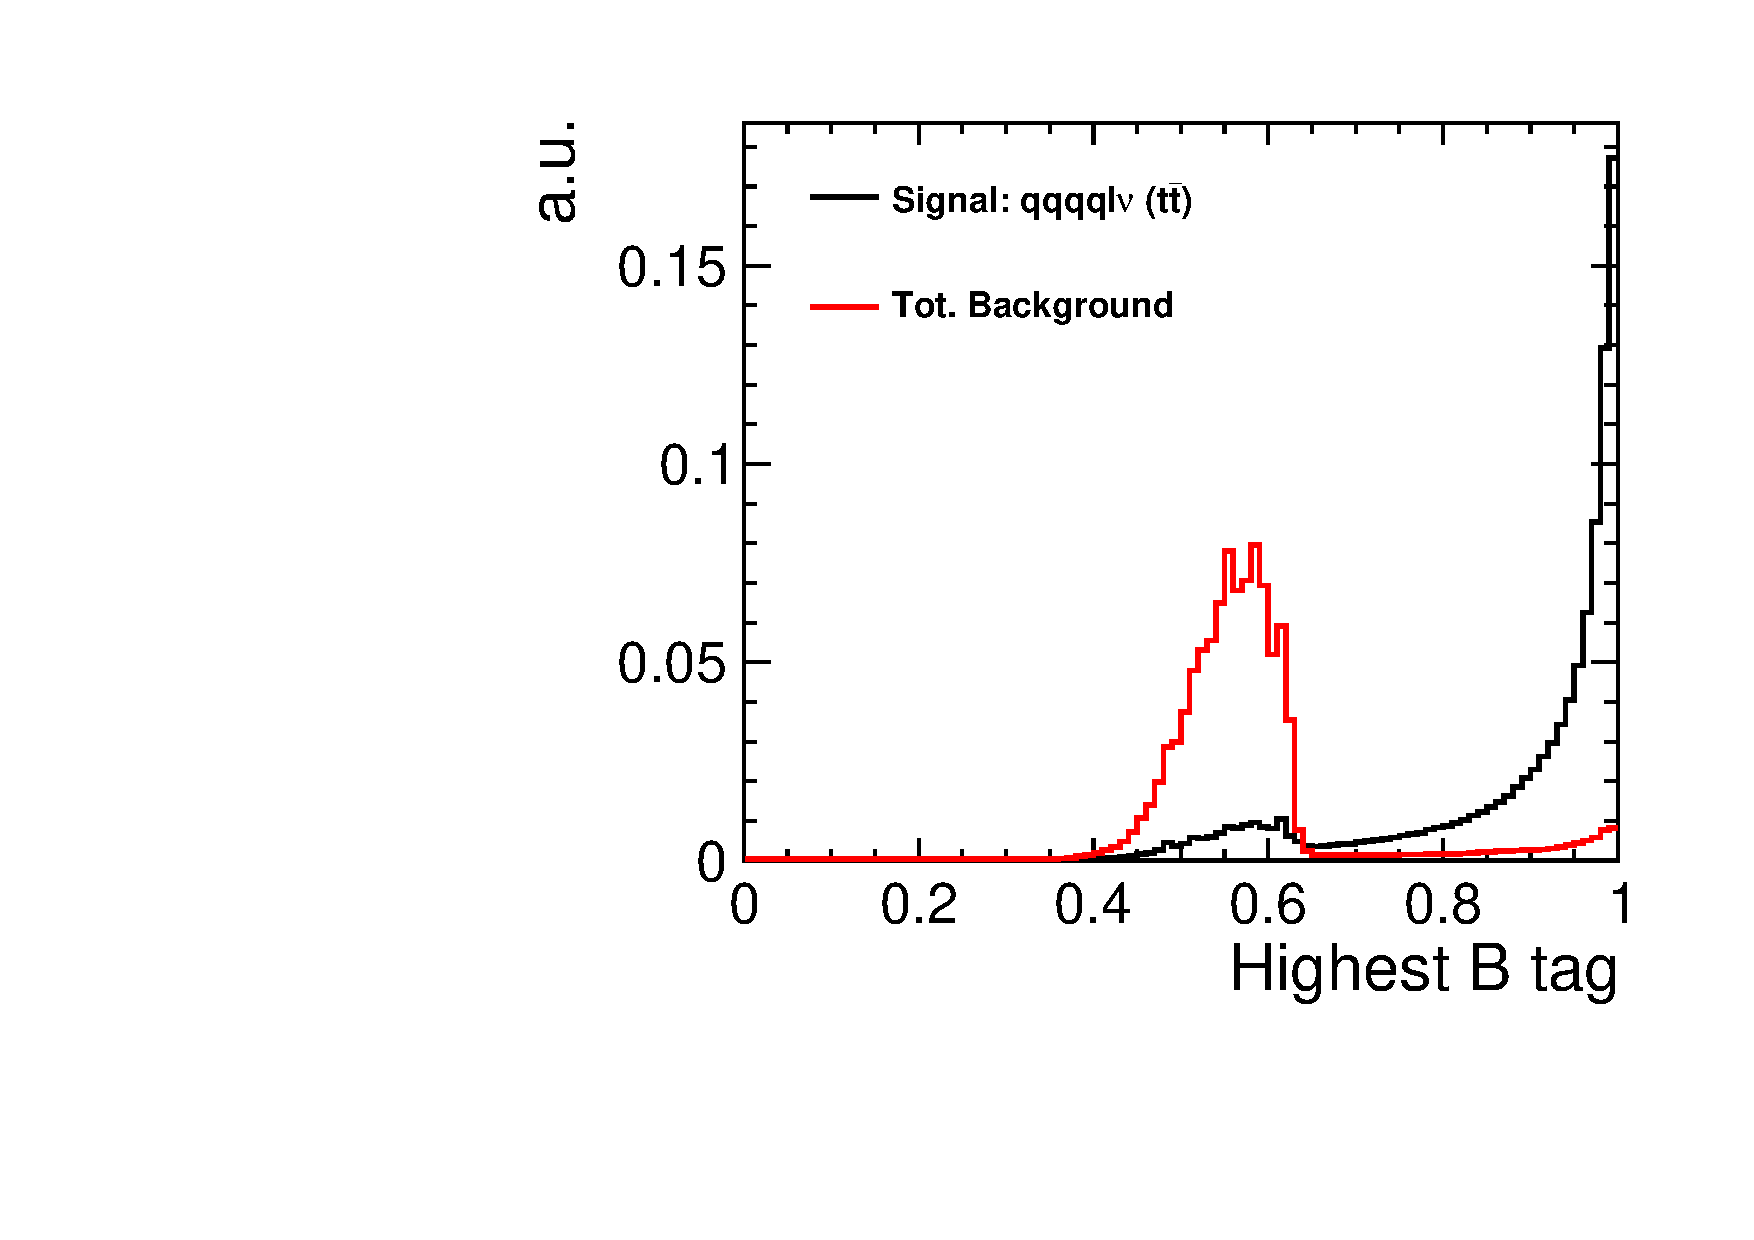
\includegraphics[width=0.75\linewidth]{TopAnalysis/figures/BDTVariables/HighestBTag.pdf} 
    \caption{Highest B tag} 
    \vspace{4ex}
  \end{subfigure}
\end{figure}

\begin{figure}[]\ContinuedFloat 
  \begin{subfigure}[b]{0.5\linewidth}
    \centering
    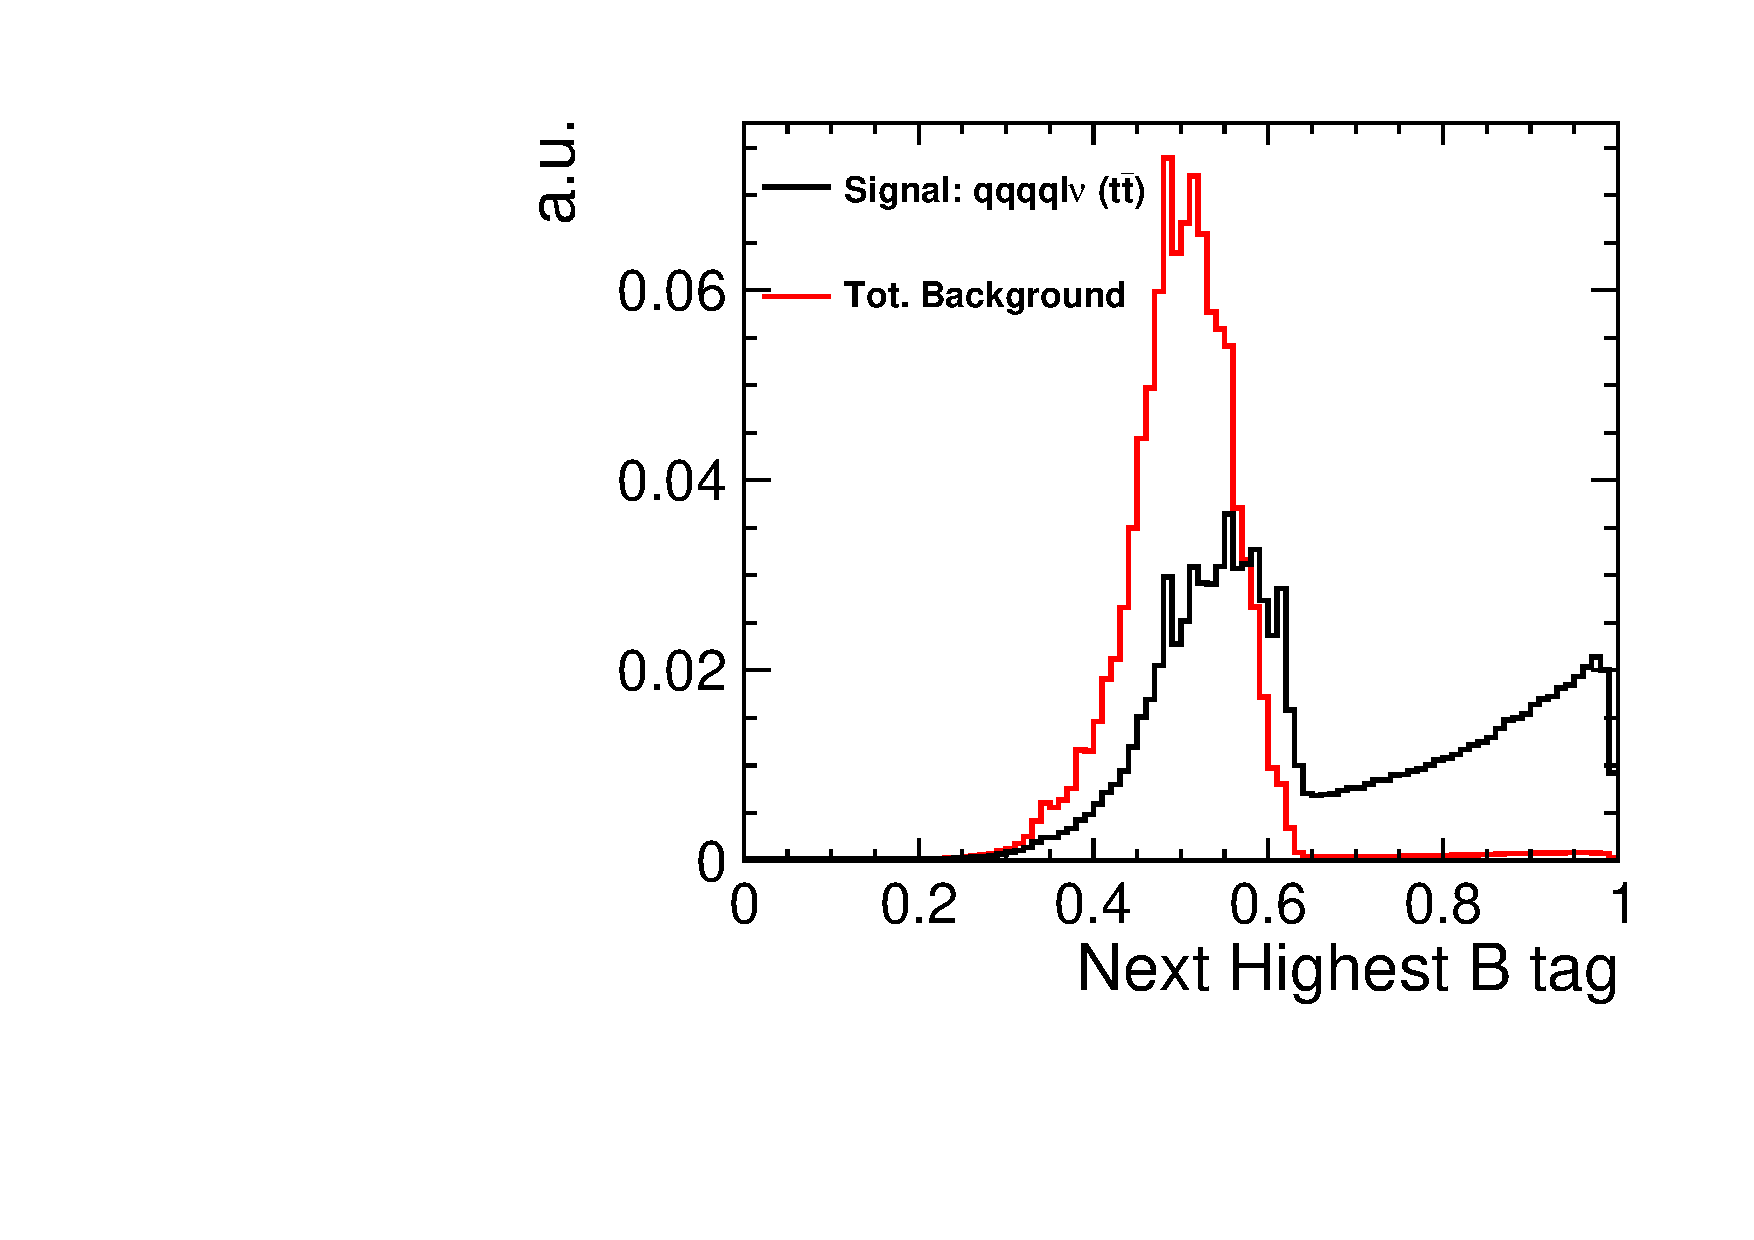
\includegraphics[width=0.75\linewidth]{TopAnalysis/figures/BDTVariables/NextHighestBTag.pdf} 
    \caption{Second Highest B tag} 
    \vspace{4ex}
  \end{subfigure} 
\end{figure}

\begin{table}
  \centering
  \begin{tabular}{l | c | c | c | c}
    \toprule
     Process     & Cross Section & Efficiency & Efficiency & N Expected\\
     & (fb) & Presel. \& Quality & BDT & \\
     \midrule
    $e^+e^-\rightarrow t\bar{t} \rightarrow qqqql\nu (l=e,\mu)$&  &  & &\\
    900$<$E$<$1200 GeV & 11.0 & 3.33E-1 & 2.85E-1 & 2350\\
    E$<$900, E$>=$1200 GeV & 35.8 & 6.31E-2 & 5.03E-2 & 1250 \\
    \midrule
    $e^+e^-\rightarrow t\bar{t} \rightarrow qqqql\nu (l=\tau)$& 23.2 & 1.03E-1  & 3.55E-2 & 620 \\
    \midrule
    $e^+e^-\rightarrow t\bar{t} \rightarrow qqqql\nu (non ~ t\bar{t})$& 72.3 & 3.71E-2 & 1.83E-2 & 990\\
    \midrule
    $e^+e^-\rightarrow qqqqqq$ & 116.4 & 2.45E-2 & 1.95E-3& 170 \\
    \midrule
    $e^+e^-\rightarrow qql\nu l\nu$ & 44.1 & 3.00E-2 & 1.87E-2 & 620\\
    \midrule
    $e^+e^-\rightarrow qqqq$ & 2304.0 & 2.39E-3 & 5.23E-5 & 90 \\
    \midrule
    $e^+e^-\rightarrow qql\nu$ & 6975.0 & 4.17E-4& 1.33E-5& 70 \\
    \midrule
    $e^+e^-\rightarrow qqll$ & 2681.0 & 2.40E-4& 1.53E-5 & 30 \\
    \midrule
    $e^+e^-\rightarrow qq\nu\nu$ & 1395.0 & 9.10E-5 & 1.27E-5 & 10 \\
    \midrule
    $e^+e^-\rightarrow qq$ & 4843.0 & 1.83E-3 & 8.03E-5 & 290\\
    \midrule
    \midrule
    TotalBackground & 18500 & 1.60 E-3 & 3.06E-4&  4246 \\
    \bottomrule
  \end{tabular}
  \caption{Efficiency for signal and background processes being classified as 900$<$E$<$1200 GeV following all stages of selection, and the expected number of events for 750 fb$^-1$ for -80\% polarization}
  \label{table:topfinalefficienciesnegMidE}
\end{table}

\begin{table}
  \centering
  \begin{tabular}{l | c | c | c | c}
    \toprule
    Process     & Cross Section & Efficiency & Efficiency & N Expected\\
         & (fb) & Presel. \& Quality & BDT & \\
    \midrule
    $e^+e^-\rightarrow t\bar{t} \rightarrow qqqql\nu (l=e,\mu)$ &  & \\
    900$<$E$<$1200 GeV & 5.8 & 3.02E-1 & 2.57E-1 & 1120\\
    E$<$900, E$>=$1200 GeV & 18.9 & 5.46E-2& 4.45E-2& 630\\
   \midrule
    $e^+e^-\rightarrow t\bar{t} \rightarrow qqqql\nu (l=\tau)$& 12.3 & 9.54E-2 & 2.62E-2& 240\\
    \midrule
    $e^+e^-\rightarrow t\bar{t} \rightarrow qqqql\nu (non ~ t\bar{t})$& 16.5 & 9.54E-2 & 3.27E-2 & 510\\
    \midrule
    $e^+e^-\rightarrow qqqqqq$ & 44.9 & 2.80E-2 & 2.03E-3 & 70 \\
    \midrule
    $e^+e^-\rightarrow qql\nu l\nu$ & 15.3  & 4.84E-2 & 2.70E-2 & 310 \\
    \midrule
    $e^+e^-\rightarrow qqqq$ & 347.0 & 3.88E-3 & 1.24E-4 & 30 \\
    \midrule
    $e^+e^-\rightarrow qql\nu$ & 1644.0 & 2.08E-4& 1.78E-5 & 20\\
    \midrule
    $e^+e^-\rightarrow qqll$ & 2529.0 & 1.63E-4 & 1.11E-5 & 20 \\
    \midrule
    $e^+e^-\rightarrow qq\nu\nu$ & 180.0 & 1.62E-4 & 2.31E-5 & 3 \\
    \midrule
    $e^+e^-\rightarrow qq$ & 3169.0 & 1.42E-3 & 9.16E-5 & 220 \\
    \midrule
    \midrule
    TotalBackground & 7980 & 1.56E-3& 3.26E-4&  1950 \\
    \bottomrule
  \end{tabular}
  \caption{Efficiency for signal and background processes being classified as 900$<$E$<$1200 GeV following all stages of selection and the expected number of events for 750 fb$^-1$ for +80\% polarization}
  \label{table:topfinalefficienciesposMidE}
\end{table}


\begin{table}
  \centering
  \begin{tabular}{l | c | c | c | c}
    \toprule
     Process     & Cross Section & Efficiency & Efficiency & N Expected\\
     & (fb) & Presel. \& Quality & BDT & \\
     \midrule
    $e^+e^-\rightarrow t\bar{t} \rightarrow qqqql\nu (l=e,\mu)$&  &  & &\\
    400$<$E$<$900 GeV & 16.6 & 4.00E-2 & 3.62E-2 & 450\\
    E$<$400, E$>=$900 GeV & 30.2 & 4.90E-3 & 3.88E-3 & 90\\
    \midrule
    $e^+e^-\rightarrow t\bar{t} \rightarrow qqqql\nu (l=\tau)$& 23.2 & 6.49E-3 & 2.94E-3 & 50 \\
    \midrule
    $e^+e^-\rightarrow t\bar{t} \rightarrow qqqql\nu (non ~ t\bar{t})$& 72.3 & 4.16E-3 & 2.56E-3 & 140\\
    \midrule
    $e^+e^-\rightarrow qqqqqq$ & 116.4 & 2.63E-3 & 4.51E-4 & 40 \\
    \midrule
    $e^+e^-\rightarrow qql\nu l\nu$ & 44.1 & 6.75E-3 & 4.90E-3 & 160\\
    \midrule
    $e^+e^-\rightarrow qqqq$ & 2304.0 & 1.67E-4 & 7.65E-6 & 10 \\
    \midrule
    $e^+e^-\rightarrow qql\nu$ & 6975.0 & 5.14E-5 & 1.73E-6 & 10 \\
    \midrule
    $e^+e^-\rightarrow qqll$ & 2681.0 & 4.09E-5 & 5.12E-6 & 10 \\
    \midrule
    $e^+e^-\rightarrow qq\nu\nu$ & 1395.0 & 1.09E-5 & 3.64E-6 & 4 \\
    \midrule
    $e^+e^-\rightarrow qq$ & 4843.0 & 1.53E-4 & 1.52E-5 & 60\\
    \midrule
    \midrule
    TotalBackground & 18500 & 1.52E-4 & 4.12E-5 & 570  \\
    \bottomrule
  \end{tabular}
  \caption{Efficiency for signal and background processes being classified as 400$<$E$<$900 GeV following all stages of selection, and the expected number of events for 750 fb$^-1$ for -80\% polarization}
  \label{table:topfinalefficienciesnegLowE}
\end{table}

\begin{table}
  \centering
  \begin{tabular}{l | c | c | c | c}
    \toprule
    Process     & Cross Section & Efficiency & Efficiency & N Expected\\
         & (fb) & Presel. \& Quality & BDT & \\
    \midrule
    $e^+e^-\rightarrow t\bar{t} \rightarrow qqqql\nu (l=e,\mu)$ &  & \\
    400$<$E$<$900 GeV & 8.7 & 5.00E-2 & 4.59E-2 & 300\\
    E$<$400, E$>=$900 GeV & 16.0 & 5.10E-3 & 4.17E-3 & 50\\
   \midrule
    $e^+e^-\rightarrow t\bar{t} \rightarrow qqqql\nu (l=\tau)$& 12.3 & 6.53E-3 & 3.27E-3 & 30\\
    \midrule
    $e^+e^-\rightarrow t\bar{t} \rightarrow qqqql\nu (non ~ t\bar{t})$& 16.5 & 6.32E-3 & 4.63E-3 & 60\\
    \midrule
    $e^+e^-\rightarrow qqqqqq$ & 44.9 & 2.89E-3 & 4.81E-4 & 20 \\
    \midrule
    $e^+e^-\rightarrow qql\nu l\nu$ & 15.3  & 1.33E-2 & 8.55E-3 & 100 \\
    \midrule
    $e^+e^-\rightarrow qqqq$ & 347.0 & 3.27E-4 & 4.67E-5 & 10 \\
    \midrule
    $e^+e^-\rightarrow qql\nu$ & 1644.0 & 4.36E-5 & 7.93E-6 & 10\\
    \midrule
    $e^+e^-\rightarrow qqll$ & 2529.0 & 2.22E-5 & 5.54E-6 & 10 \\
    \midrule
    $e^+e^-\rightarrow qq\nu\nu$ & 180.0 & 1.16E-5 & $<$E-6 & 10 \\
    \midrule
    $e^+e^-\rightarrow qq$ & 3169.0 & 7.40E-5 & 5.84E-6 & 10 \\
    \midrule
    \midrule
    TotalBackground & 7970 & 1.35E-4 & 4.98E-5 & 300\\
    \bottomrule
  \end{tabular}
  \caption{Efficiency for signal and background processes being classified as 400$<$E$<$900 GeV following all stages of selection and the expected number of events for 750 fb$^-1$ for +80\% polarization}
  \label{table:topfinalefficienciesposLowE}
\end{table}


